\chapter{X線CT}



\section{X線CTとは}
\begin{wrapfigure}{r}{90mm}
 \begin{center}
 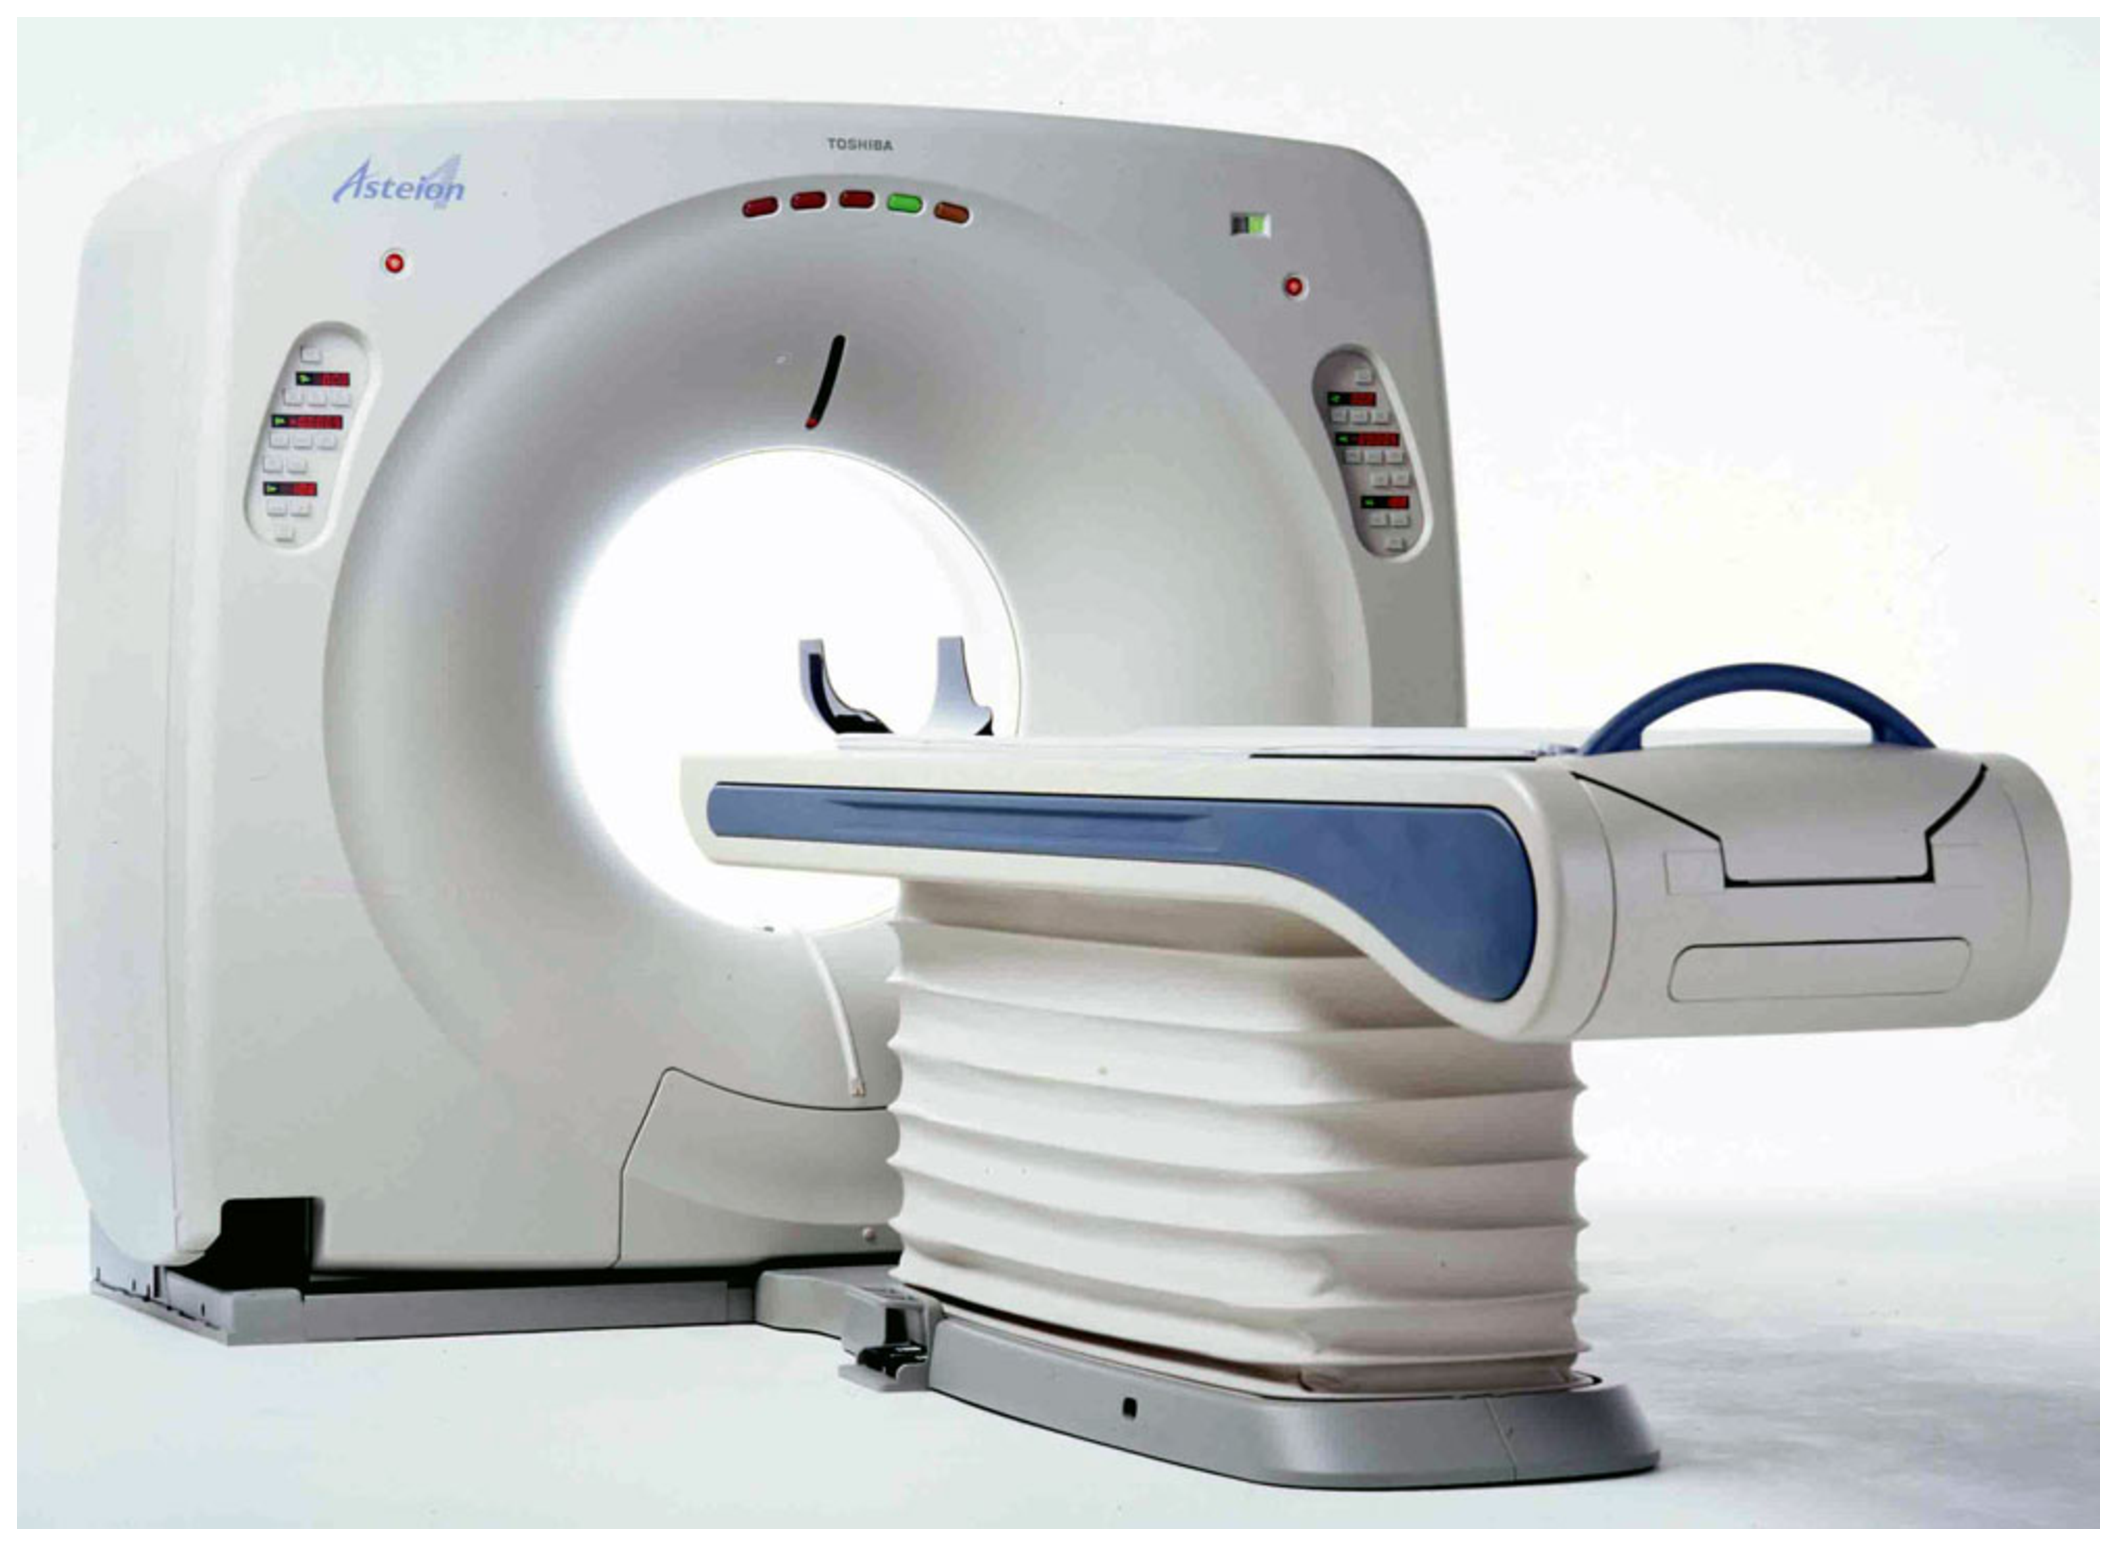
\includegraphics[width=8cm]{image/other/CT_toshiba.eps}
 \end{center}
 \caption{CT装置の外観}
 \label{fig:CT_toshiba}
\end{wrapfigure}
CTとはcomputed\ tomographyの略であり,日本語名称はコンピュータ断層撮影装置である。\Fref{fig:CT_toshiba}が典型的なCTの外観例である。X線管から連続エネルギースペクトルを持つX線が照射され,直進しながら物体中で減弱し,反対側にある検出器で減弱したX線の透過強度分布を測定する。そして,測定した透過強度分布から,X線の通しにくさを影絵にしたような投影データを取得する。この投影データをX線管と検出器を物体周りに回転して物体の多方向から取得し,フーリエ変換を用いて画像再構成し線減弱係数$\mu$の分布図としてCT画像を表示している。CT画像においては線源弱係数の高い組織は白く,線源弱係数の低し組織は黒く表示するのが慣例である。CTの方式には種々の方式があるが現在最も一般的なのは第三世代のファンビームを照射するX線源とそれに対向したX線検出器が被写体の周りを回るRotate/Rotate(R/R)方式であり,X線検出素子の数(チャンネル数)は現在は700-900程度になっており一回転のスキャン時間は0.3秒前後に達している。\\


\ \ 現在実用化されているCTの仕様の一例を\Tref{CT_philips}に示す。解像度は$\sim$0.2mm,画像を取得するのに要する時間は100ミリ秒台である。
\begin{table}[H]
\begin{center}
\begin{tabular}{cc} \hline
項目 & 仕様 \\\hline
フレームレート & 10,000 frame/sesc($\sim$120,000pixel/frame) \\
動作モード & 電流モード(エネルギー積分型) \\
シンチレータ & GOS($\sim$50,000ph/MeV) \\
解像度 & $\sim$2.4lp/mm($\sim$0.210mm) \\
リーク電流 & $<3$pA \\\hline
\end{tabular}
\end{center}
\caption{PHILIPS市販されているCTの仕様\cite{philips}}
\label{CT_philips}
\end{table}



\section{X線CTの検出器}
CTのX線検出器にシンチレータとフォトダイオード(PD)が用いられ、シンチレータでX線を光に変換し、PDで光電変換を行うのが最も主流である。シンチレータにはX線阻止能が高く、発光量が大きく、残光が少ないGOSが用いられる。また、R/R方式においては検出器全面に高さ20-30mmの主にタングステンなどの重金属でできている散乱線カット用のコリメータが配備されている。\Fref{fig:colimater}。
また、PDからの出力電流をサンプリング時間(1ビューの時間、つまり0.2$\sim$1 ms)について積分し、たまった電荷量をA-D変換しディジタルデータとして送り出すDAS(Data Acquisition System)の構成の一例を\Fref{fig:DAS}に示す。DASに求めらる性能は以下のようなものがある。
\begin{enumerate}
\item サンプリング時間(0.2$\sim$1 ms)内に全検出素子の出力をA-D変換する高速性。
\item 検出器・DAS系の回路ノイズと量子化誤差はX線量子の統計的変動より十分低いレベルでなければならない
\item 被写体による減弱がない場合でも簡単にオーバーフローしない広いダイナミックレンジを持つ。
\end{enumerate}



また,CTの動作モードには電流モード(X線フォトンによって生成した電荷を所定時間蓄積し,電流信号を出力する方式)とパルス読み出し(X線フォトンを個々に計数するフォトンカウンティングモード)の2種類に大別されるが通常のCTは電流モード読み出しでありエネルギー積分型と呼ばれる。





\section{画像再構成原理}
現在のX線CTのX線管からはファンビームのX線が照射されるのが一般的であるが,ここでは簡単のため直線のX線ビームを用いて画像再構成原理を説明する(\Fref{fig:FBP})。

\begin{wrapfigure}{l}{60mm}
 \begin{center}
 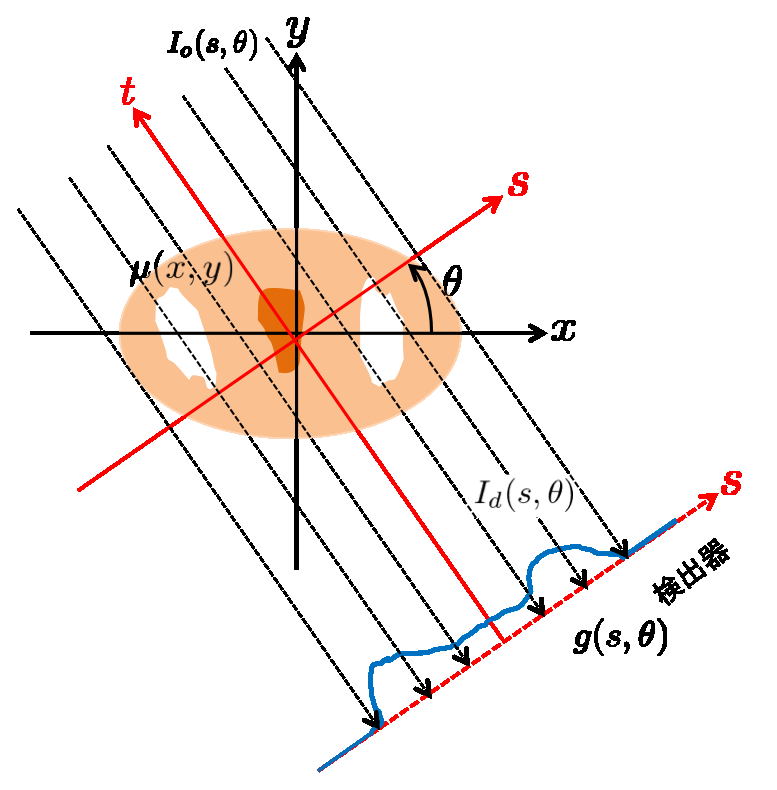
\includegraphics[width=6cm]{image/other/FBP.eps}
 \end{center}
 \caption{CTの画像再構成法の原理}
 \label{fig:FBP}
\end{wrapfigure}

最終的な目標は線源弱係数の分布$\mu(x,y)$を求めることである。投影データとはX線パス$s$に沿って$\mu(x,y)$を線積分した値として以下のように定義される。
\begin{align}
&p(t,\theta)=\int\mu(x,y)ds\\
&(t=x\cos{\theta}+y\sin{\theta})
\end{align}
各$\theta$と$t$で規定される投影データ1本1本をレイ(ray)という。まあ一つの角度方向のレイの1セットをビュー(view)という。投影データの値は入射強度$I_0$と検出器で受ける強度$I_d$とから求められる\footnote{入射強度$I_0(t,\theta)$は直接計測できないが,この値はキャリブレーション補正により計測しない済む仕組みになっている。}。\Eref{eq:atten}より

\begin{align}
I_d(t,\theta)&=I_0(t,\theta)\exp{\left[-\int\mu(x,y)ds\right]}\\
&=I_0(t,\theta)\exp[-p(t,\theta)]\\
∴p(&t,\theta)=-\ln\left[\frac{I_d(t,\theta)}{I_0(t,\theta)}\right]\label{eq:touei}
\end{align}
つまり,投影データ$p(t,\theta)$を入射強度$I_0$と検出器で受ける強度$I_d$から求めることができれば,その逆変換として,$\mu(x,y)$を求めることができる。そこで$\mu(x,y)$の二次元フーリエ変換$\hat{\mu}(\xi,\eta)$を考えると

\begin{align}
\hat{\mu}(\xi,\eta)=\displaystyle\int^{\infty}_{-\infty}\int^{\infty}_{-\infty}\mu(x,y)e^{-i(\xi x+\eta y)}dxdy
\end{align}となり,$(\xi,\eta)$を$\xi=\omega\cos{\theta},\eta=\omega\sin{\theta}$なる変換を行い,極座標系$(\omega,\theta)$に変換すると,

\begin{align}
\hat{\mu}(\omega\cos{\theta},\omega\sin{\theta})&=\int^{\infty}_{-\infty}\int^{\infty}_{-\infty}\mu(x,y)e^{-i\omega(x\cos{\theta}+y\sin{\theta})}dxdy\\&=\int^{\infty}_{-\infty}\int^{\infty}_{-\infty}\mu(x,y)e^{-i\omega t}dtds\\
&=\int^{\infty}_{-\infty}\left[\int^{\infty}_{-\infty}\mu(x,y)ds\right]e^{-i\omega t}dt\\
&=\int^{\infty}_{-\infty}p(t,\theta)e^{-i\omega t}dt\label{eq:mu_hat}
\end{align}
つまり\Eref{eq:mu_hat}はある角度$\theta$における投影データを$t$について一次元フーリエ変換したものは線減弱係数$\mu$の二次元フーリエ変換の$\theta$成分である。よって,投影データを$\theta$が0から$\pi$に対して$\theta$方向\footnote{平行ビームであれば$p(t,\theta+\pi)=p(-t,\theta)$なので半回転で投影データの情報完備となる。画像の安定化のためには1回フルスキャンが基本だが,理論の説明は半回転の方がつ都合がよい。}の成分を得てそれらをtに関して1次元フーリエ変換することにより,$\mu(x,y)$のフーリエ空間$\hat{\mu}(\xi,\eta)$をタイヤのスポーク状に埋めることにより$\hat{\mu}(\xi,\eta)$が求まることになる。よって線源弱係数の分布$\mu(x,y)$は\Eref{eq:mu_hat}を逆フーリエ変換すればよいので
\begin{align}
\mu(x,y)=\frac{1}{(2\pi)^2}\int^{\infty}_{-\infty}\int^{\infty}_{-\infty}\hat{\mu}(\xi,\eta)e^{i(\xi x+\eta y)}d\xi d\eta
\end{align}
と求まる。CT画像の画素の値はこの線源弱係数を用いて以下のように定義されている。

\begin{align}
\rm CT値=1000\times\frac{\mu-\mu_w}{\mu_w}\label{eq:CT_value}
\end{align}
ここでCT値の単位はHU(Hounsfield\ unit)であり,$\mu_w$は水の線源弱係数である。しかし,$\mu$も$\mu_w$もX線質に依存する量であり,混合エネルギーX線を用いているため,物質を透過するとX線質は変化するのでCT値は完全な定量的な値ではない。様々な物質のCT値の目安を\Fref{fig:CT_value}に示す。

\begin{figure}[H]
 \begin{center}
 \includegraphics[bb=0.000000 0.000000 400.000000 140.000000,width=0.8\hsize]{image2/chapter1/CT_value.jpg} 
 \end{center}
 \caption{様々な物質のCT値}
 \label{fig:CT_value}
\end{figure}

※フィルターの話、ランプフィルターとシェップローガン

\section{CTの画質評価}
CTの画質評価に主にどれくらい画像ノイズ評価、どれくらい細いものが見えるかという空間分解能表、CT値が近い物質をどれくらい区別できるかという低コントラスト分解能評価お3つが主にある。

\subsection{画像ノイズ評価}
X線CTで水ファントムのような一様な被写体を撮影した場合、その物質の線減弱係数$\mu$に従って、各ピクセルのCT値は一様に等しく計算されるはずである。しかし、実際は諸因子に由来する統計的な変動(揺らぎ)によってCT値はばらついて一定とならず、この揺らぎ成分を一般的に画像ノイズと呼ぶ。この画像ノイズは直感的にも推察されるように投影データのノイズの比例する。ここでは投影データのノイズはX線量子の統計的変動が支配的である。X線量子の統計的変動とは次のようなものである。完全な計測系を用いて到来フォロン数の計測を繰り返しても、結果は毎回異なる。個々のX線フォトンが被写体内で減弱していくプロセスは確率現象であるためであり、一般的にポアソン分布に従うと仮定される。各回のフォトン数計測値が$N$個であるとし、平均して$\langle N \rangle$個が計測されたとする。$N$は$\langle N \rangle$を中心に誤差$\varepsilon_N$でばらつくが、この$\varepsilon_N$がX線量子の統計的変動である。$\varepsilon_N$の標準偏差を$\sigma_N$とすれば、ポアソン分布を仮定しているので$\sigma_N=\sqrt{\langle N \rangle}$である。誤差のない測定系であっても計測データのS/N比はX線量子の統計的変動で決まる物理限界$\langle N \rangle/\sigma_N=\sqrt{\langle N \rangle}$を超えることはできない。\\
ここで、検出器・DASは完璧でなくノイズ$\varepsilon_d$を伴うが、その場合の投影データのノイズレベルを求めてみる。CTのX線計測は様々なエネルギーの混じった混合エネルギースペクトルの多色X線の吸収線量計測であるが、ここでは簡単のためにフォトンカウンティングモードでの計測であるとする。被写体へ入射X線フォトン数を$N_{\rm in}$とする。\Eref{eq:touei}よりノイズがなければ投影データの値は
\begin{align}
p_{\rm ideal}&=-\ln{\left(\frac{N}{N_{\rm in}}\right)}\\
&=-\ln{N}+\ln{N_{\rm in}}\\
&=-\ln{\langle N \rangle}+\ln{\langle N_{\rm in} \rangle}
\end{align}
ノイズがあるときの投影データは
\begin{align}
p_{\rm actual}&=-\ln{\left( \frac{N+\varepsilon_d}{N_{\rm in}}   \right)}\\
&=-\ln{(N+\varepsilon_d)}+\ln{N_{\rm in}}\\
&=-\ln{(\langle N \rangle + \varepsilon_N + \varepsilon_d)}+\ln{(\langle N_{\rm in} \rangle + \varepsilon_{\rm in})}
\end{align}
ここで、$\varepsilon_{\rm in}$は$N_{\rm in}$に含まれるX線量子の統計的変動でありその標準偏差は$\sqrt{\langle N_{\rm in} \rangle}$であるが、$N_{\rm in}$は被写体により減弱していない大きな値なので$\langle N_{\rm in} \rangle\gg|\varepsilon_{\rm in}|$であり、$\ln{\langle N_{\rm in} \rangle + \varepsilon_{\rm in}}\approx\ln{\langle N_{\rm in} \rangle}$と近似してよい。従って
\begin{align}
p_{\rm actual}&\approx-\ln{(\langle N \rangle + \varepsilon_N + \varepsilon_d)}+\ln{\langle N_{\rm in} \rangle}\\
&=-\ln\left\{\langle N \rangle\left(1+\frac{\varepsilon_N+\varepsilon_d}{\langle N \rangle} \right)\right\}+\ln{\langle N_{\rm in} \rangle}\\
&=-\ln{\langle N \rangle}-\ln\left(1+\frac{\varepsilon_N+\varepsilon_d}{\langle N \rangle} \right)+\ln{\langle N_{\rm in} \rangle}\\
\end{align}
ここで第ニ項を級数展開し$\langle N \rangle$に比べて$\varepsilon_N$と$\varepsilon_d$は十分小さいとして高次の項を落とすと、
\begin{align}
p_{\rm actual}&\approx-\ln{\langle N \rangle}-\frac{\varepsilon_N+\varepsilon_d}{\langle N \rangle}+\ln{\langle N_{\rm in} \rangle}\\
&=p_{\rm ideal} + \varepsilon_p
\end{align}
ここで
\begin{align}
\varepsilon_p\equiv-\frac{\varepsilon_N+\varepsilon_d}{\langle N \rangle}
\end{align}
と定義した。すなわち$p_{\rm actual}$は$p_{\rm ideal}$の周囲に誤差$\varepsilon_p$でばらつく。この$\varepsilon_p$の標準偏差$\sigma_p$を求める。ここで$\varepsilon_d$は平均値ゼロ、標準偏差$\sigma_d$とする。$\varepsilon_N$と$\varepsilon_d$とは互いに相関がないので分散の加算式より、

\begin{align}
\sigma^2_p&=\frac{\sigma^2_N+\sigma^2_d}{\langle N \rangle^2}\\
&=\frac{\langle N \rangle + \sigma^2_d}{\langle N \rangle^2}
\end{align}
従って
\begin{align}
\langle N \rangle\gg\sigma_dのとき\ \ \ \sigma_p\approx\frac{1}{\sqrt{\langle N \rangle}}\label{eq:normal}\\
\langle N \rangle\ll\sigma_dのとき\ \ \ \sigma_p\approx\frac{\sigma_d}{\sqrt{\langle N \rangle}}\label{eq:ijou}
\end{align}
\Eref{eq:normal}が通常の運用状態である。ここではX線量子の統計的変動だけが投影データ(すなわちCT画像の)ノイズ起源で画像ノイズは検出線量の平方根に反比例する。\\
\Eref{eq:ijou}のような状況では、画像ノイズは検出線量に反比例して変化する。これは一種の異常事態であり、大きな被写体であるにもかかわらず過度に照射線量を減らしたり薄いコリメーション幅とした場合には発生しうる。その場合、画像ノイズのみならず別種の画質問題も顕在化することがあり、診断に耐える画像は得られない。

\if0
%森田バージョン
X線CTで水ファントムのような一様な被写体を撮影した場合、その物質の線減弱係数$\mu$に従って、各ピクセルのCT値は一様に等しく計算されるはずである。しかし、実際は諸因子に由来する統計的な変動(揺らぎ)によってCT値はばらついて一定とならず、この揺らぎ成分を一般的に画像ノイズと呼ぶ。この画像ノイズは直感的にも推察されるように投影データのノイズの比例する。ここでは投影データのノイズはX線量子の統計的変動が支配的である。X線量子の統計的変動とは次のようなものである。完全な計測系を用いて到来フォロン数の計測を繰り返しても、結果は毎回異なる。個々のX線フォトンが被写体内で減弱していくプロセスは確率現象であるためであり、一般的にポアソン分布に従うと仮定される。各ピクセルの投影データの値は\Eref{eq:touei}から求められるが、X線量子の統計的変動によって$I_d/I_o$が揺らぎ、投影データの値も揺らぐことになる。極端な線量不足による電気系のノイズが顕在化する場合を除き、X線量子数を$n$とすると、投影データの値の揺らぎつまりピクセルごとのCT値の揺らぎ($SD$)は
\begin{align}
SD\propto\frac{1}{\sqrt{n}}
\end{align}

このように、CT値の変動はX線量子数の平方根に反比例し、このX線量子数は管電流時間積[mAs]または管電圧[kV]によって調整可能である。一般的にCT検査ではほとんどの場合、管電圧は120kVカラ140kVの一定の値あが使用されるため、管電流や撮影時間を調整することで画像ノイズをコントロールするこができる。
\fi


\subsection{空間分解能評価}
空間分解能とはどのくらい細いものを分離して認識できるかという識別限界を数値化したものである。CTにおける空間分解能は、高コントラスト分解能ファントムを用いて視覚的に評価する方法と、解像特性として定量的に変調伝達関数(Modulation Transfer Function: MTF)を測定する方法の2つが推奨されている。空間分解能を決定づける要因は以下のようなものがあげられる。
\begin{enumerate}
\item 焦点サイズと検出器サイズ
\item サンプリングピッチ
\item view数
\item 再構成FOV
\item 再構成関数
\item その他(架台振動、管球焦点移動なども影響がある。マルチスライスCTの登場により再構成方法も多様化し、これらの様々な要因によっても空間分解能が変化する。)
\end{enumerate}

\subsection{高コントラスト分解能ファントムによる空間分解能評価}
一般的な評価ファントムとしては、\Fref{fig:high_contrast_phantom}のようにアクリル樹脂などの中に空気の穴(直径$d$)がピッチ$2d$で配列されたものが用いられる。これをCT撮影して再構成を行い画像上で$d$の穴が分離して見えるか見えないかという主観的な評価を行う。この評価においては定量性には欠けるが穴が細くなる、つまり入力信号の周波数が大きくなるにつれて応答性が次第に低下していることなどもわかる。例えば0.5mmの径であれば、空間周波数1.0 Lp/mmにおける応答を見ていることになる。下がって、それぞれの径に対応する空間周波数における応答を比較することができる。しかし、本法では空間周波数ごとの応答を定量的な数値で表すことはできず、本法で評価してるのは識別限界となる最高周波数のみである。

\subsection{MTFによる空間分解能評価}
上述の高コントラスト分解能ファントムによる評価では、「どのくらい細いものを分離して認識できているか」という主観的な視覚評価であった。一方で変調伝達関数(Modulation Transfer Function: MTF)では「見える、見えない」といった主観的な要素はなう、また周波数領域について定量的、客観的に評価が行える。MTFとは入力信号に対して、出力信号が「どれだけボケたか」を周波数成分ごとに数値化したものである。MTFを求める入力信号としては、店信号を入力する点像強度分布(Point Spread Function : PSF)と線信号を入力する線像強度分(Line Spread Function : LSF)がある。ここでは最も一般的な手法であるワイヤ法という、スライス面と垂直に張ったごく細い金属ワイヤの断面をCTで撮像し、得られたPSFからMTFを求める手法について詳細に述べる。\\
PSFから求めるMTFとは「何もないところに突然ある限りなく0に近い幅で無限大のCT値を持つ入力信号」が「どのようにボケたのか」ということを示したものである。この場合の極めて特殊な入力信号をインパルス信号と呼ぶ。「どのようにボケたのか」ということを評価するために、ボケによって得られた分布すなわちPSFをフーリエ変換す流ことで周波数空間における応答値が得ることができる。インパルス波形を理想的なデルタ関数とすれば、これをフーリエ変換すると全周波数領域で大木さは1となる(\Fref{fig:delta})。デルタ関数を扇形システムい入力したときの出力をインパルス応答という。システムを通過したときのボケにより広がった形状のインパルス応答をフーリエ変換したものが周波数応答関数であり、その絶対値がMTFである。\\
デルタ関数をフーリエ変換した時の全周波数領域での大きさが1であることから、広がった形状のインパルス応答をフーリエ変換して得られた応答値は、ボケによって低下したレベルや、微小構造描出のために特定の周波数を強調しているような状況が周波数成分ごとにその比率としてMTF上に示される。\\
CTに於いてはスライス面と垂直に張ったごく細いワイヤは、ワイヤのある位置においてX線がほとんど不透過であるので、線減弱係数は非常に大きくなる。よって、ワイヤーの径が非常に小さければ、それによって近似的な2次元のインパルス信号が得られ(\Fref{fig;inpulse}(左))、その信号がCTシステムによってボケを受けた出力信号がCT画像上に現れたワイヤの画像、すなわちPSFである(\Fref{fig;inpulse}(右))。このPSFを直接2次元フーリエ変換するか、LSFに変換して1次元フーリエ変換をsして周波数応答を求めるのがワイヤ法である。\Fref{fig:MTF_outou}は、3種類のLSFに対するMTFを示している。この図では、幅が狭く急峻なLSFほど高いMTFとなっており、直感的にもわかりやすい。この幅が狭くなり最後にインパルス信号そのものになれば、MTFは高周波成分まで1.0となり理想的な状態となる。



\subsection{低コントラスト分解能評価}

\section{従来のエネルギー積分型X線CTの問題点\label{sec:problem}}

第1章でも述べたがフォトダイオードの暗電流は 数十pA$\sim$数百pAであり、この暗電流に十分打ち克つ信号電流を検出器から出力する必要がある。CTの画質を律速しているのは「信号電流($I_s$)$\gg$暗電流($I_d$)」を実現することに他ならない。ここで従来のCTにおいて「$I_s\gg I_d$」を実現させるために必要な照射線量を概算してみる。被写体透過後のX線強度を$I_x$[/s]、PDの暗電流$I_d$を100[pA]とする。60keVのX線が従来一般的に用いられるGOSシンチレータ(40,000 ph/MeV)に検出されたとし、PDの量子効率を50\%すると、
\begin{align}
I_d&\gg I_s\\
60\time40\times0.5\times1.6\times10^{-19} [C] \times I_x&\gg100\times10^{-12}\\
I_x&\gg 5.2\times10^5
\end{align}
程度となる。また読み出し回路を通ることでさらにノイズが増大することを考えれば被写体を透過した時点で$10^{6}$cts/s/mm$^2$のレートが必要になる。人体透過後は線量は約1/1000になるので\footnote{人体を水と透過と考え60keVにおける水の線減弱係数は0.206[1/cm]、人体を30cmとすれば$e^{-\mu L}\sim1/1000$となる。}必要な照射線量は$10^{8-9}$cts/s/mm$^2$と膨大になる。このためX線CTによる医療被ばく量は膨大であり一回の撮影での被ばく量は10mSvにもおよぶ。また、このような超高線量下おいては様々なエネルギーの混ざった混合エネルギーのX線のそれぞれの反応パルスイベントを区別するのは困難であり、読み出し方法はある一定時間電荷を積分した電流モードである。そのため個々のX線光子のエネルギー情報は完全に失われてしまう。\\




先述のように,従来のX線CTでは透過X線の検出において,電流モードつまりX線フォトンによって生成した電荷を所定時間蓄積し,電流信号を出力する方式を用いている。そのため従来型X線CTは「エネルギー積分型」と呼ばれ,各エネルギーのX線光子がどれくらい透過してきたのかというエネルギー情報は失ってしまう。しかし,人体中の元素は低原子の組織が中心であるため,X線の減弱は原子番号に依存するコンプトン散乱が支配的であるため,混合エネルギーのX線は低・高エネルギーでもある物質中で一定の割合で減衰するため線質はあまり変化しない。したがって,透過物質の実効エネルギーに対する線源弱係数はある程度正確に求めることができる。そのため長年にわたって個々のX線光子のエネルギーの計測は行われなかった。しかし,以下に述べる2点がCT誕生時からの問題点として挙げられる。

\subsection{CT値が同一である物質の弁別が困難}
CT値は,物質の「質量減弱係数」と「密度」の積である線源弱係数により決定されることを述べた。質量減弱係数はX線エネルギーが一定であれば物質固有の値(\Fref{fig:atten}左)であるが,CT値を決定する線減弱係数は物質の密度にも依存するため,撮像対象物の密度状態によっては物質が異なっても(原子番号が異なっても)CT値が同一になってしまうことがある(\Fref{fig:atten}右)。通常のCTでは,CT値が唯一のパラメータであるため,物質の正確な弁別は困難と言える。

\begin{figure}[H]
 \begin{minipage}{0.52\hsize}
  \begin{center}
   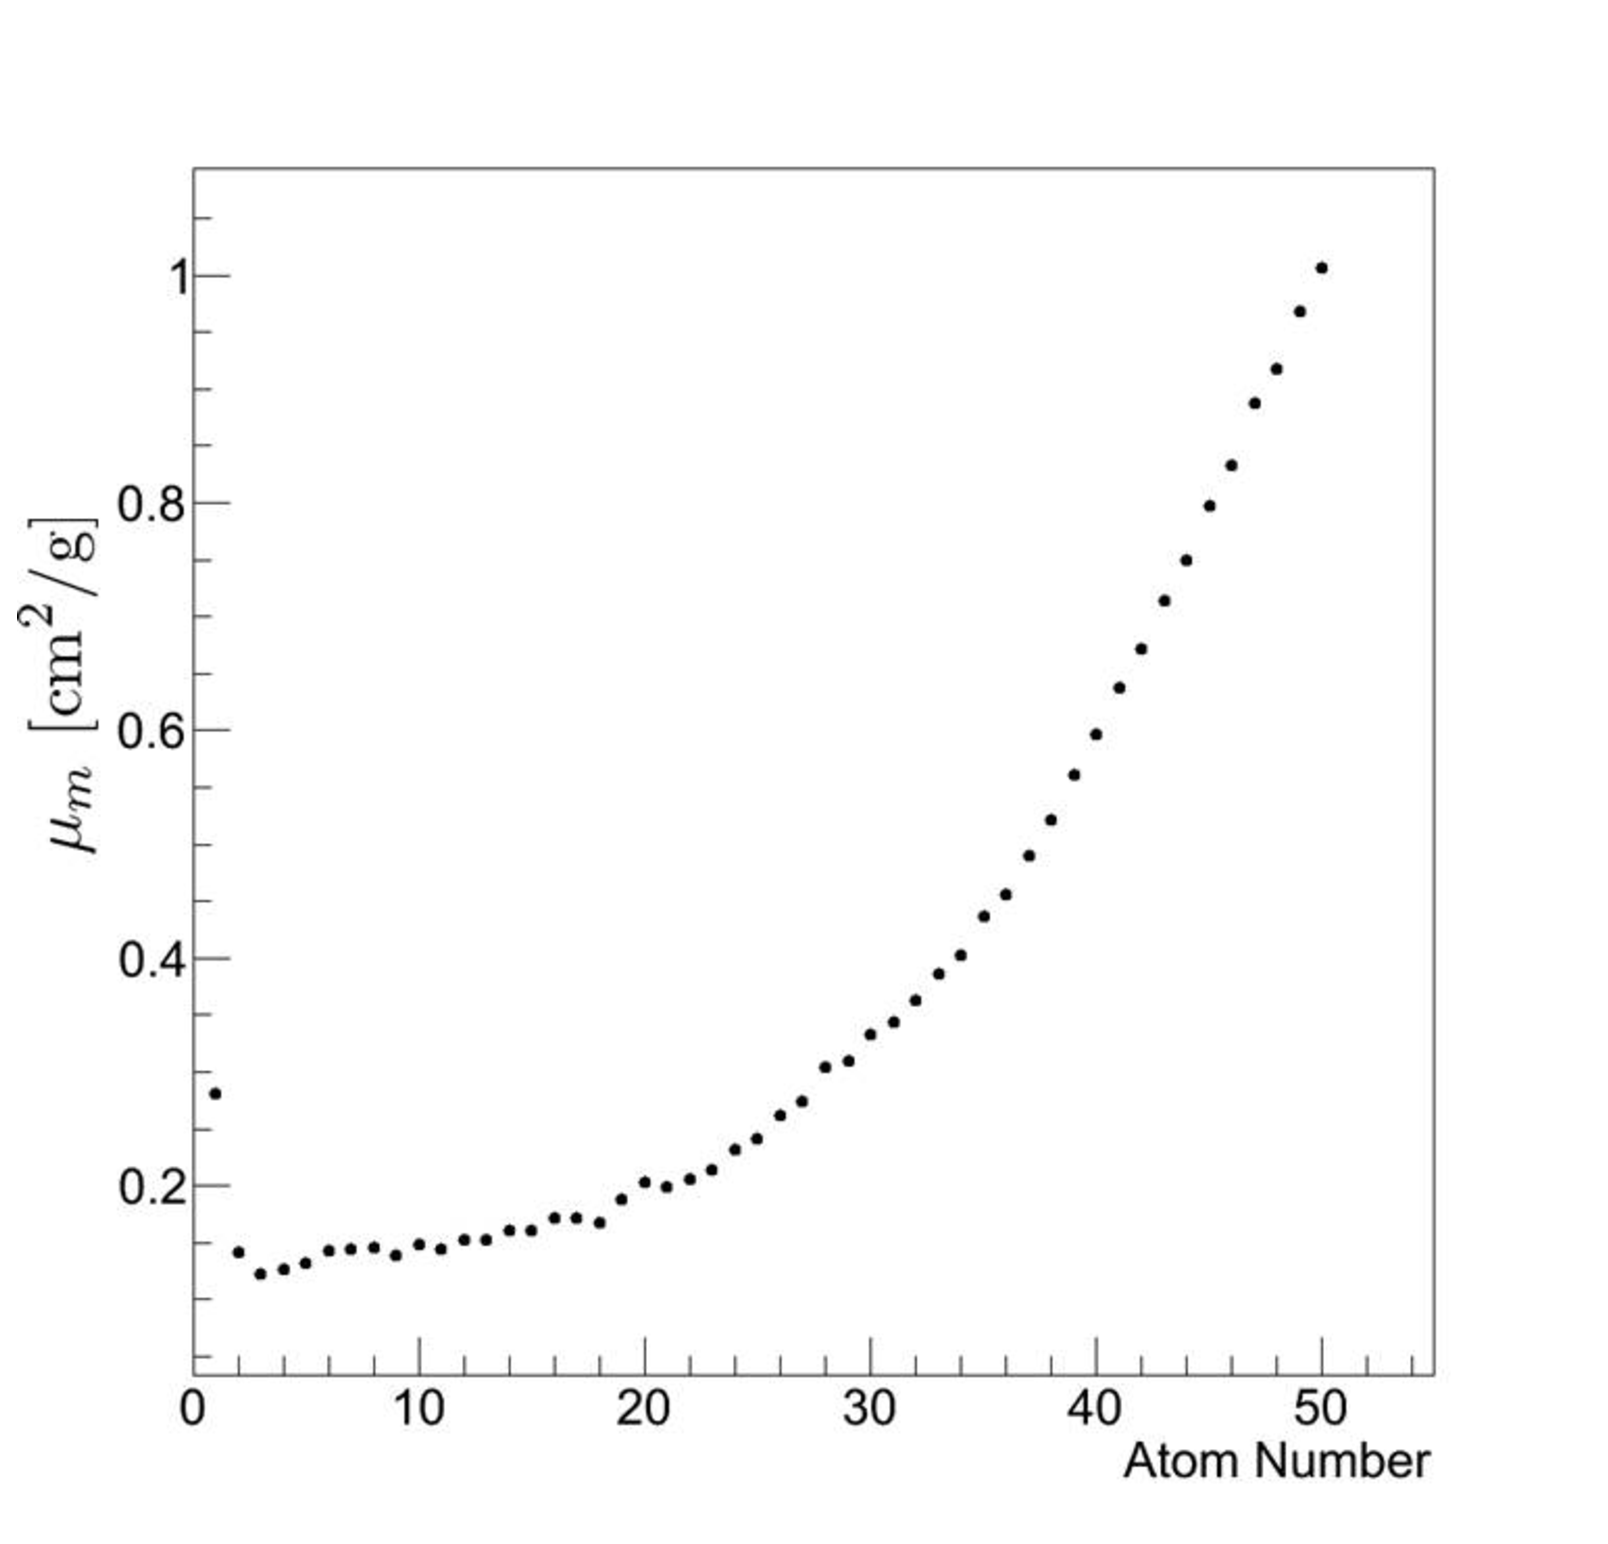
\includegraphics[width=7cm]{image/other/mass_atten.eps}
  \end{center}
 \end{minipage}
 \begin{minipage}{0.3\hsize}
  \begin{center}
   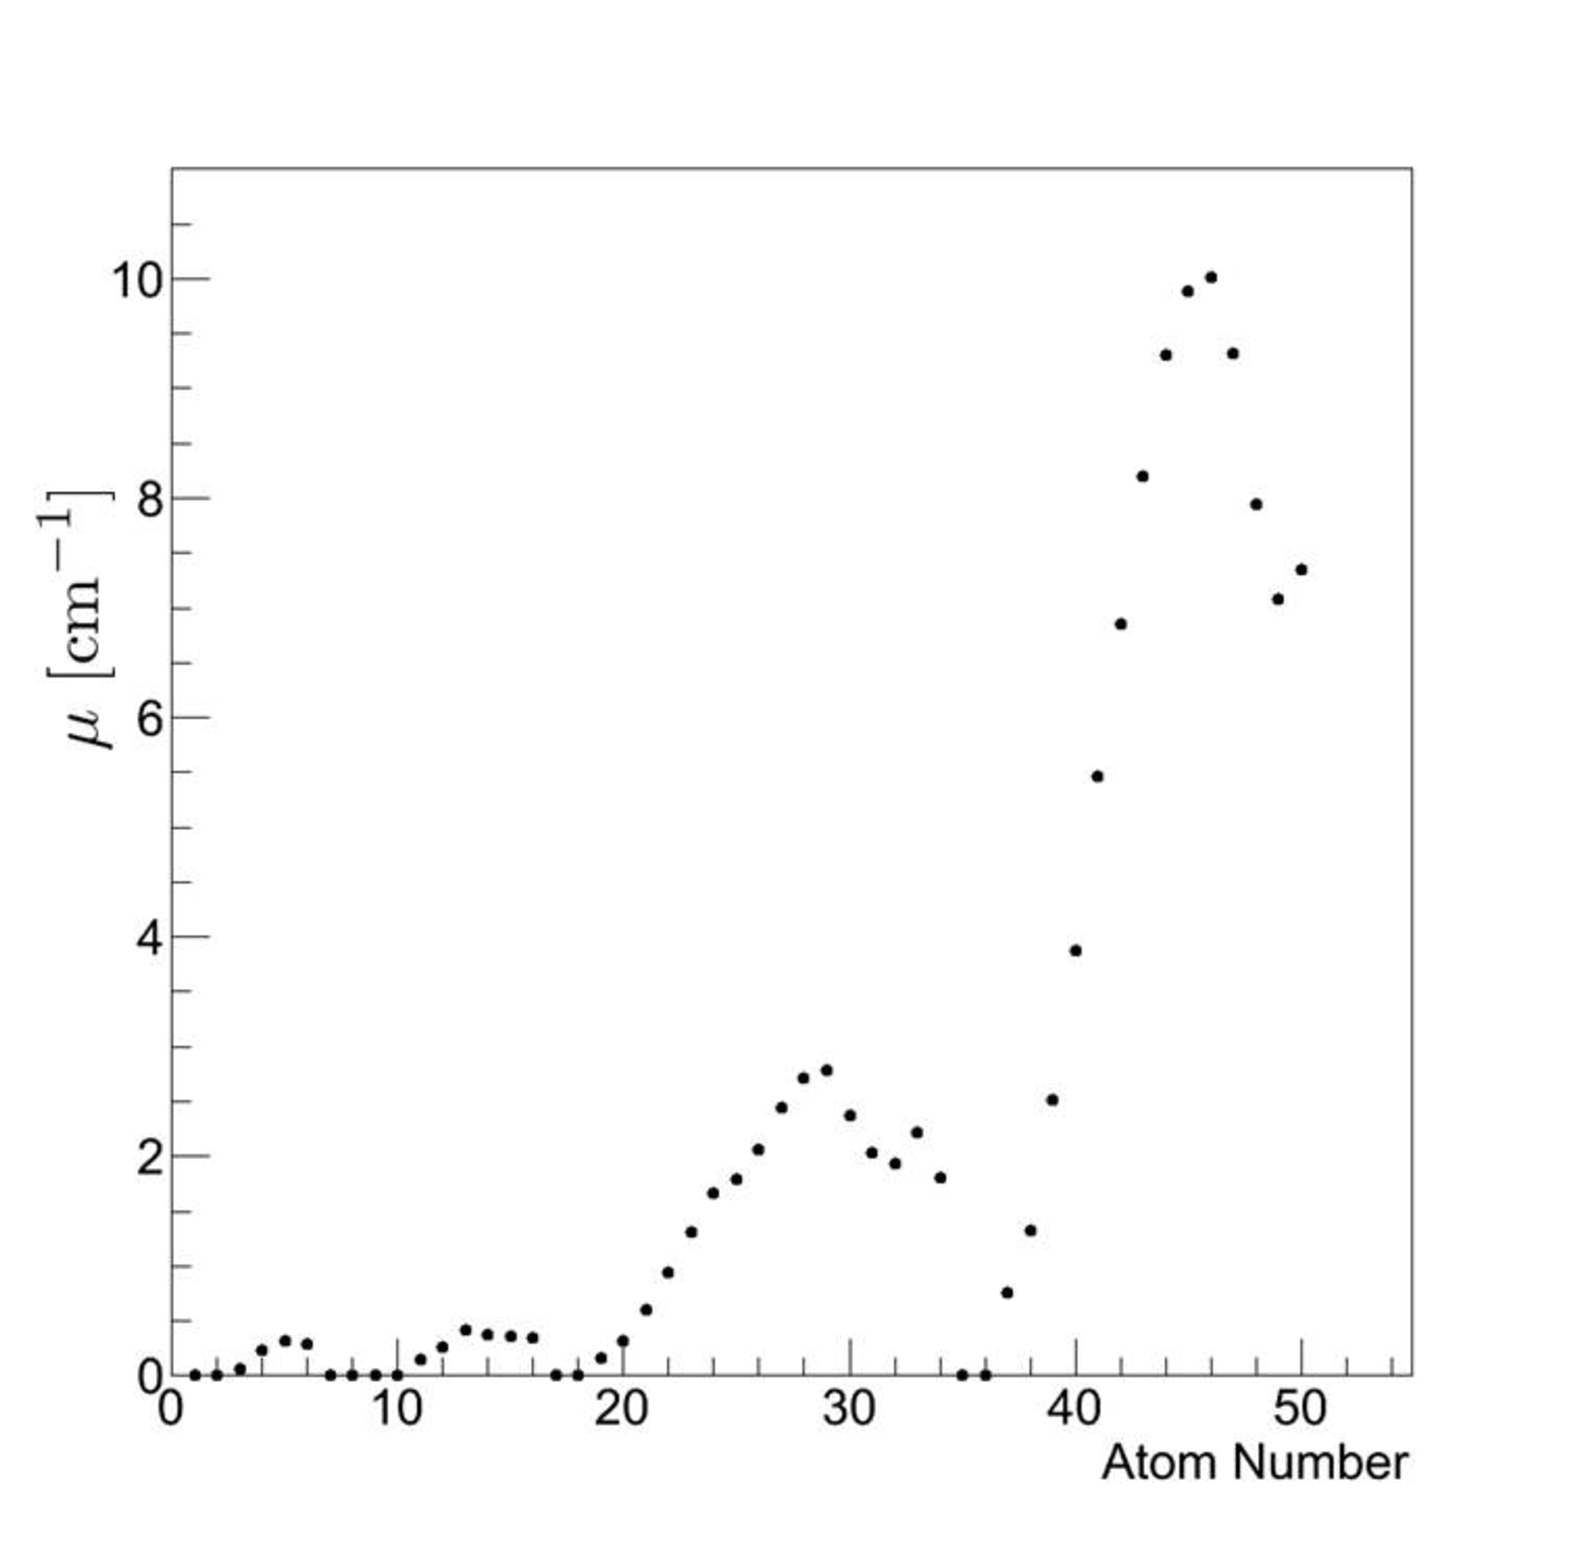
\includegraphics[width=7cm]{image/other/linear_atten.eps}
  \end{center}
 \end{minipage}
 \begin{center}
  \vspace{-1zh}
  \caption{質量減弱係数の原子番号依存性と線源弱係数の原子番号依存性(@122keV)\newline 質量減弱係数はエネルギーが一定であれば物質によって異なる値を取るが,線源弱係数は物質が異なっても同一になる場合がある}
  \label{fig:atten}
  \end{center}
\end{figure}


\subsection{ビームハードニングアーチファクト}
人体中の元素は低原子の組織が中心であるが骨の原子番号は他の組織に比べて高いため,光電効果による減弱が支配的となり,低エネルギーのX線光子が多く吸収されることになる。すなわち,X線のエネルギー分布が高エネルギー側にシフトし,その結果,実効エネルギー\footnote{平均エネルギーの意味合いとして,しばしば実効エネルギーと表現される}が高くなる(\Fref{fig:beam_hard})。高原子番号の物質周辺では実効エネルギーが高くなったX線からその部位の線源弱係数$\mu$が算出されることによりCT値が低くなり,これがアーチファクトとして現れる。人間の体はほぼ水等価物質で構成されているが,原子番号の高い骨に囲まれた部分ではアーチファクトが生じやすい(\Fref{fig:artifact_1}(a))。

\begin{figure}[H]
 \begin{minipage}{1\hsize}
  \begin{center}
   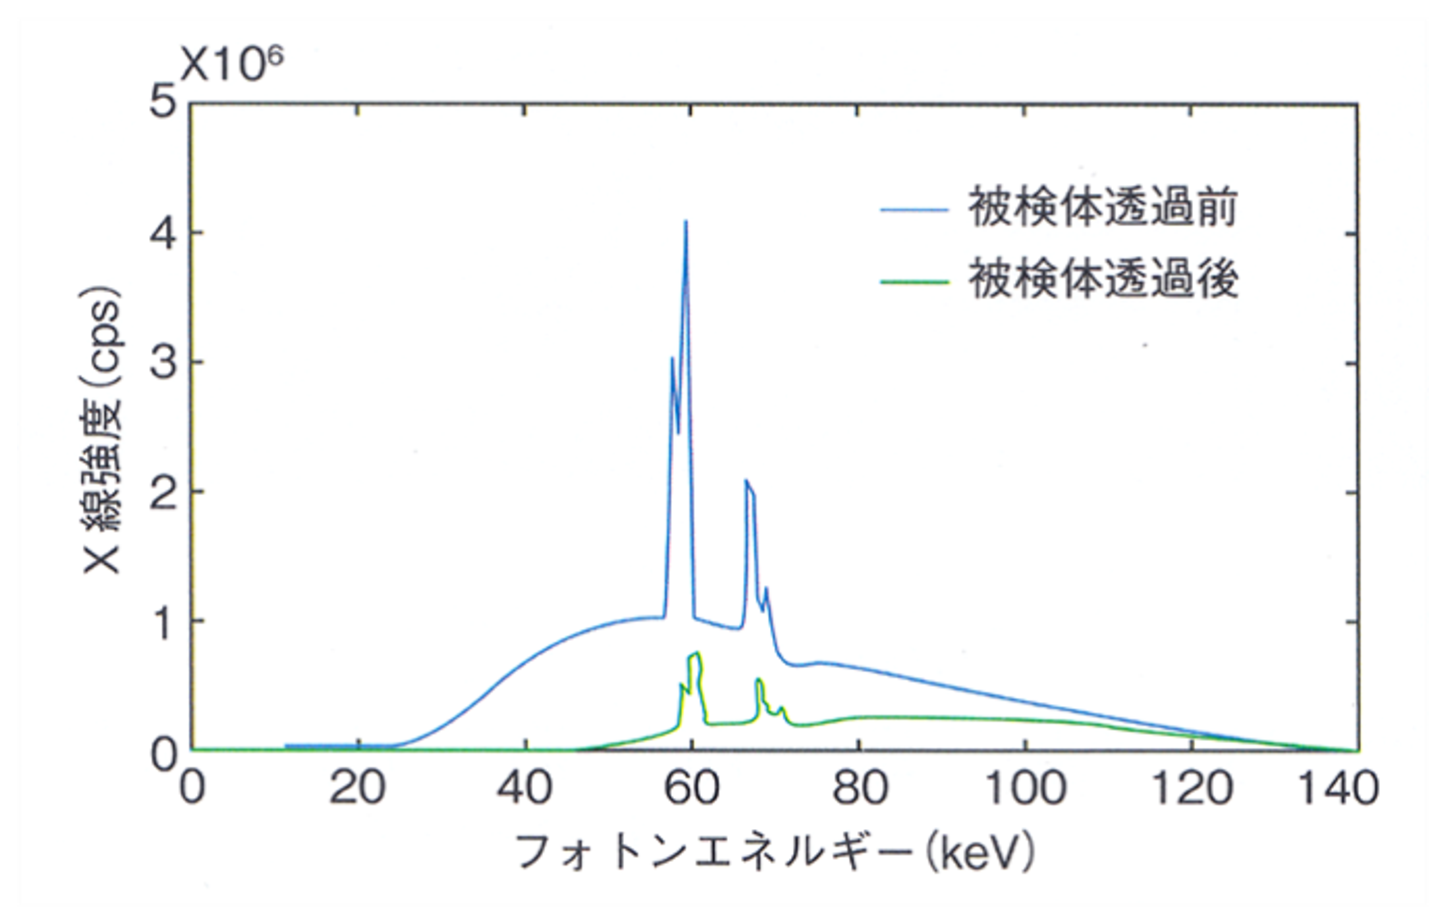
\includegraphics[width=10cm]{image/other/beam_hard.eps}
  \end{center}
  \vspace{-0.9cm}\hspace{8cm}
  
 \end{minipage}
 \begin{center}
  \vspace{-1zh}
  \caption{ビームハードニング効果\cite{spectralCT}}
  \label{fig:beam_hard}
  \end{center}
\end{figure}






\section{次世代X線CT}
上述したように通常のエネルギー積分型のCTでは,様々なエネルギーからなる混合エネルギーのX線を物質に照射し,その線源弱係数を求めCT値を画像化している。この混合したX線光子のエネルギーを分離するのは困難であり,画像化に用いられるX線エネルギーから得られる画像は1種類であるため,画像診断に用いられるパラメータはこのCT値のみとなる。その結果\ref{sec:problem}で述べたような問題が生じる。\\
\ \ そこで近年,複数のフォトンエネルギーレベルのデータを収集して画像化を行うCTが臨床応用されはじめている。このようなCTでは,画像診断に用いられるパラメータとして,複数のフォトンエネルギーレベルにおけるCT値を得ることが,通常のCTの問題点が解決される他,得られる情報が非常に多様であり通常のCTではできないイメージングが可能となる。このようなCTを次世代CTと本稿では呼ぶことにする。次世代
CTには低・高2種類の混合エネルギーのX線を照射するデュアルエナジーCTと1種類の混合エネルギーのX線を照射しパルスモード(フォトンカウンティングモード)読み出しを行うことでエネルギー帯域ごとにCT画像を取得するフォトンカウンティングCTがある。

\subsection{デュアルエナジーCT\label{sec:dual}}
デュアルエナジーCTではまず低・高2種類の混合エネルギーのX線を照射しそれぞれ別々に画像再構成する。その後,各々の画像に対して処理を施すことにより,単色X線透過画像を作成できたりと様々な画像化が可能となる。現在,実用化されているデュアルエナジーCTは以下の3方式に大別される\cite{GE}\cite{siemens}\cite{philips}。

\begin{enumerate}
\renewcommand{\labelenumi}{(\arabic{enumi})}
\item 2回転方式\\CT装置自体は通常のCTと変化しないが,1つのX線管を用い,1回転ごとに管電圧(1回転目:80kVp,2回転目:140kVp)を切り替えて撮影する方式
\item 2管球方式\\設置角度の異なる2つのX線管を用い,異なる管電圧(80kVpと140kVp)で同時に撮影する方式
\item 1管球高速kVpスイッチング方式\\1つのX線管を用い,ビュー毎に高速で管電圧を切り替えて(80kVpと140kVp)撮影する方式
\end{enumerate}

2回転方式は得られる2種類のデータの撮影時間差(時相差)が大きく,撮影時の呼吸運動や体動などの影響を受けやすく画像データ上での位置のズレなどが起こりうる。2管球方式は時相差は2回転方式に比べ短くなっているが,依然大きい(70msec)。また2つのX線管は90$^{\circ}$離れており,各検出が収集した投影データもこの管球角差$90^{\circ}$の差が反映されるため,2種類のエネルギーデータが1:1に対応しない。これらの理由によりこの2方式では投影データではなく画像データに基づいてデュアルエナジーCTの画像化を行うため,時相差によるミスレジストレーション\footnote{重ね合わせる用紙や画像などの位置ずれを示す}が生じやすい。\\
\ \ 一方,1管球高速kVpスイッチング方式は2管球ではなく1つのX線管球を用いて異なる2種類の管電圧を高速に切り替えて撮影を行うので時相差は0.5msec以下であり,管球差は当然ない。従って,時間的及び空間的にほぼ完全に一致した投影データに基づいて解析を行うことができる。現在臨床応用されているのは3つのうちこの方式のみである。投影データから解析を行うことで単色X線透過画像が取得でき既に多数の臨床応用例がある\cite{spectralCT}。

\begin{figure}[H]
 \begin{center}
 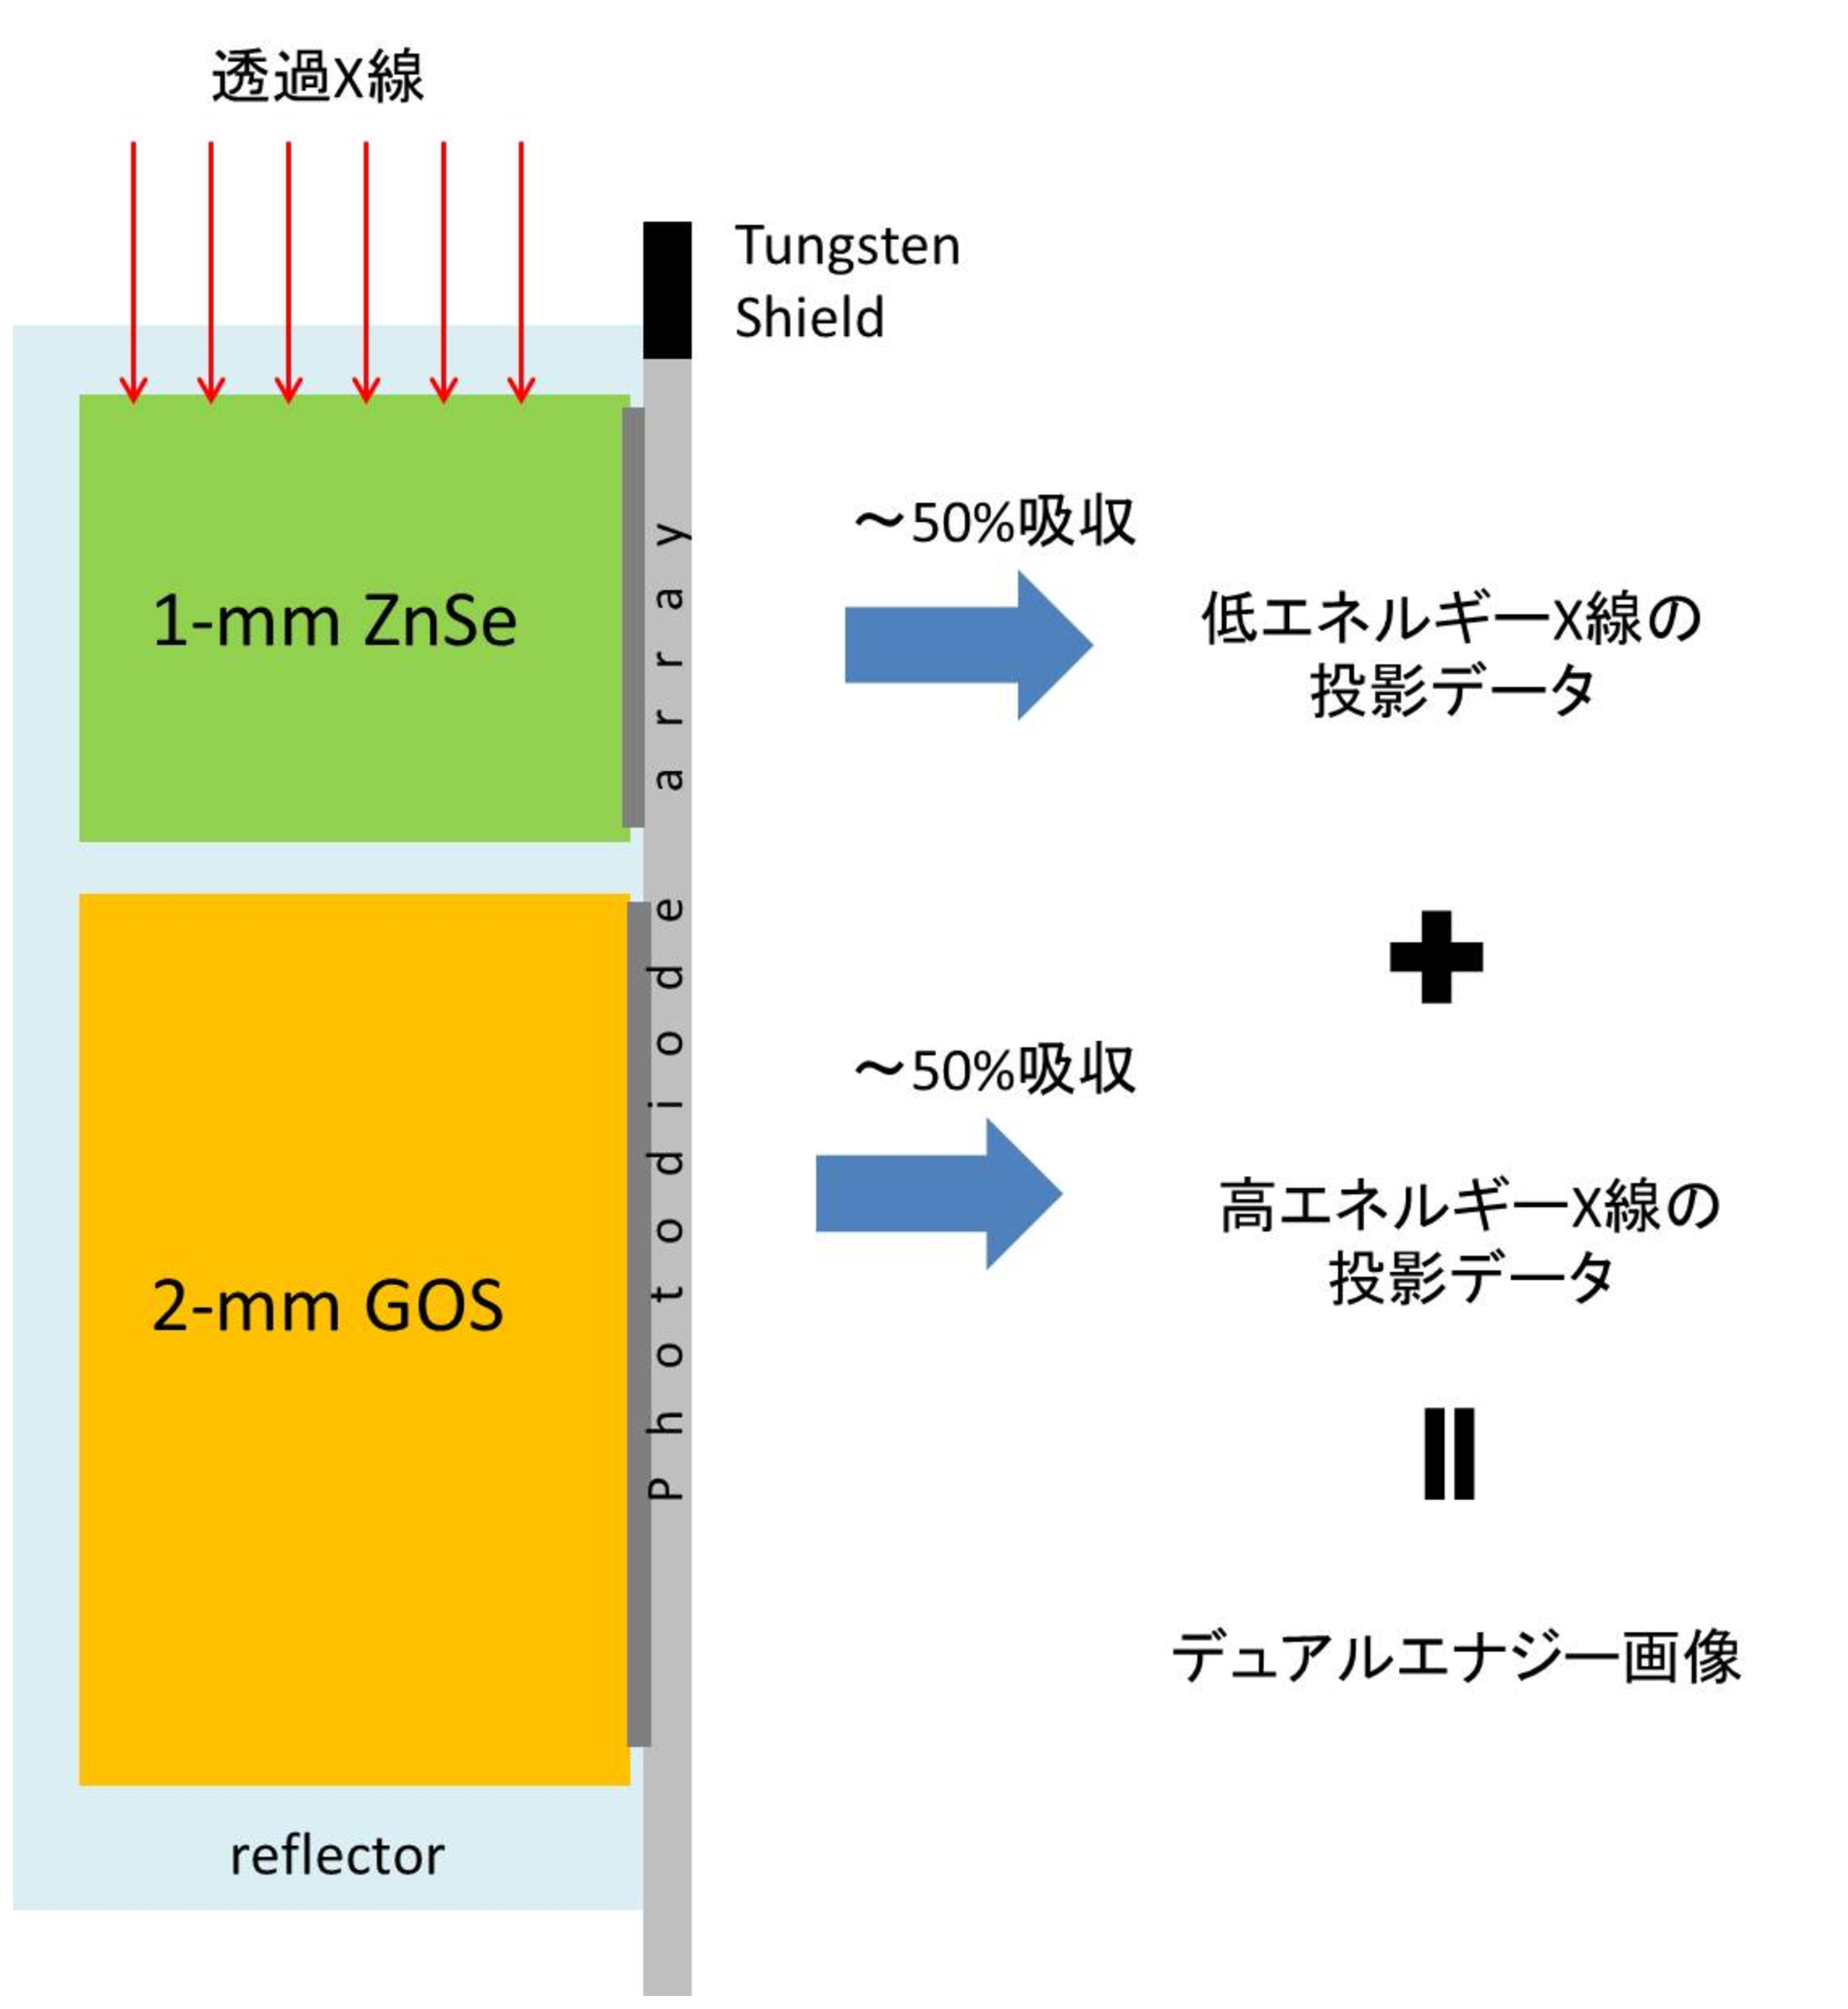
\includegraphics[width=7cm]{image/other/two_layer.eps}
 \end{center}
 \caption{2層式検出器方式\cite{philips}}
 \label{fig:two_layer}
\end{figure}

また別のアプローチのデュアルエナジーCTとして,2層式検出器方式がある(\Fref{fig:two_layer})。これは検出器は異なる材料の2層式の構造になっており,被写体を透過してきたX線はまずCsI,ZnSeなど低エネルギーにしか感度を持たない上層のシンチレータで低エネルギーのX線光子のみが吸収され,この低エネルギー成分から投影データをまず1つ作成することができる。その後,高エネルギー成分が下層の($\rm Gd_2O_2S(GOS)$)によって吸収され,高エネルギー成分のデータからもう1つ投影データを作成することが出来る。こうして低エネルギー,高エネルギーに対する2種類の投影データを作成することができ,投影データに基づいたエネルギー解析により,デュアルエナジーCTの画像化が行われる。この手法においては空間的,時間的なズレは全くなくなるが,高・低エネルギーX線を完全に二層の検出器で分けることはできず,重複領域が大きい。さらにX線上層の検出器を透過する際,大量の散乱線が生じうる,下層の検出器により得られるエネルギーデータに悪影響を及ぼす可能性があるなどの問題がある。\\\ \ 二層式の検出器は空港手荷物用のX線検査装置に利用されており実用化されている場面もある\cite{airport_1}\cite{airport_2}。

\subsection{フォトンカウンティングCT\label{sec:CT_photon}}
フォトンカウンティングCTは1つのX線管により1種類の管電圧で撮影するため,通常のCTと同様に用いるのは1種類の混合エネルギーX線のみである。この1種類の混合エネルギーX線に対して,検出器においてX線を構成する各フォトンのエネルギーが計測され,エネルギー帯域ごとに分けてカウントし,エネルギー帯域別にCT画像を出力するのがフォトンカウンティングCTである。デュアルエナジーCTでは2種類のX線を照射するので患者の被曝量は通常のCTよりも多くなるが,フォトンカウンティングCTでは1種類のエネルギーのX線のみ用いればよいため被曝量は増えず,管電圧スイッチングに伴う時相差はまったく生じない。また,フォトンカウンティングCTは各々のフォトンをエネルギー帯域別にカウントでき,マルチエナジー画像の再構成が容易である。\\
\ \ フォトンカウンティングCTを実現するためには,パルス読み出しを行う必要がある。そのためには,光検出器が高い増幅率を持ち,S/Nが高い必要がある。さらに従来のCTの画質とスピードを実現するためには10$^6$counts/sec/mm$^2$という高計数に耐えなければならない。従って,シンチレータ側には従来のCTの要求に加えてパイルアップを防ぐために減衰時間が短い必要がある。\\ 
\ \ 現在のX線CTに用いられているGOSは減衰時間が$\sim$3$\mu$sと非常に長く,高計数に対応することはできない。また増幅機能を持たないPDを用いることでノイズ耐性は低く,そもそもパルス読み出し自体が困難である。さらにPDの数が膨大なためデータ処理の面からもパルス読み出しは困難である。従ってシンチレーション検出からフォトンカウンティングCTへのアプローチではなく,エネルギー分解能が高い半導体を用いたフォトンカウンティングCTが現在のトレンドとなっている。現在最も広く研究されてい応用されているフォトンカウンティング検出器はテルル化カドミウム(CdTe)とテルル化亜鉛カドミウム(CdZnTe:CZT)素材の半導体検出器である\cite{ogawa}\cite{ogawa_id}\cite{kowase}\cite{Adam}\cite{Jan}。エネルギー分解能は$4.4\%$(FWHM@122keV)を実現している\cite{ogawa}。しかし,\ref{sec:CdTe}で述べたが,CdTeは電荷収集時間が遅く,さらに増幅機能を持たないため,長い時定数でのチャージセンシティブアンプの使用が不可欠であり,高計数には対応しないという問題がある。\\\ 以下にフォトンカウンティングCTの通常のCTと比べた場合の利点に関して述べる。

\subsubsection{ビームハードニングの低減}
スペクトラルCTではX線の投影データをエネルギー帯域別に取得するため,ビームハードニングは起こらない。エネルギー帯域ごとに取得した画像に対して高エネルギーの画像の重みを多くして画像を合成することにより,ビームハードニングのアーチファクトを低減することができる\cite{kowase}。また,実際の診断においてスペクトラルCTによるアーチファクトの低減例\cite{spectralCT}を\Fref{fig:artifact_1}と\Fref{fig:artifact_2}に示す。

\begin{figure}[H]
 \begin{minipage}{0.52\hsize}
  \begin{center}
   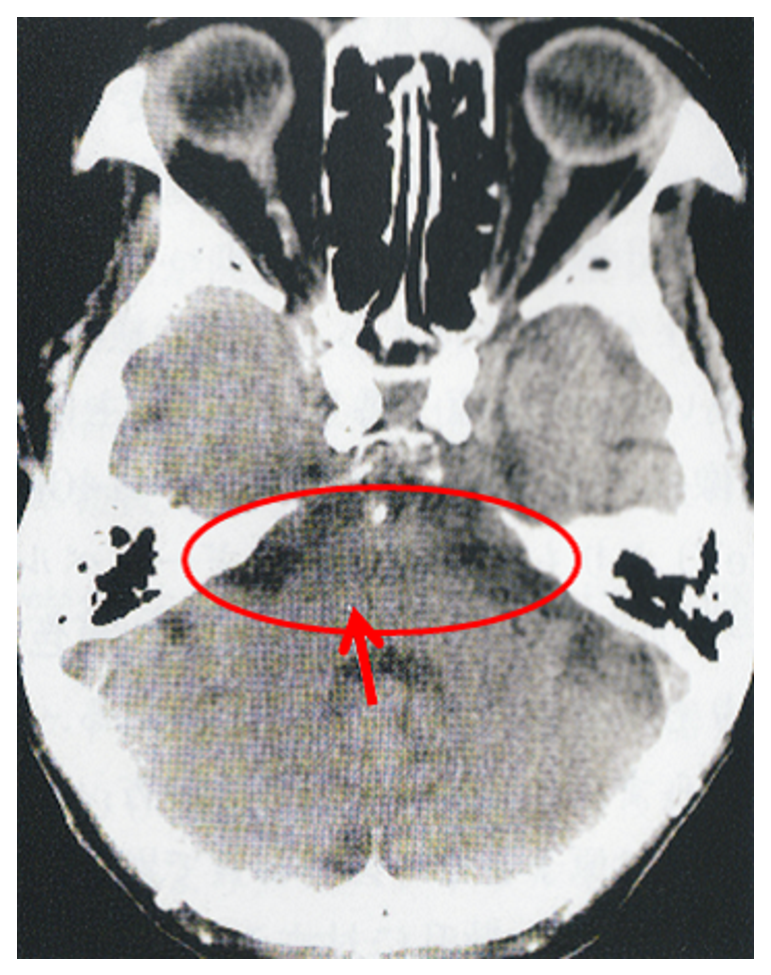
\includegraphics[width=5cm]{image/other/artifact_1.eps}
  \end{center}
  \vspace{-0.5cm}\hspace{1cm}
   (a)エネルギー積分型CT画像(140kVp)
 \end{minipage}
   \begin{minipage}{0.5\hsize}
  \begin{center}
   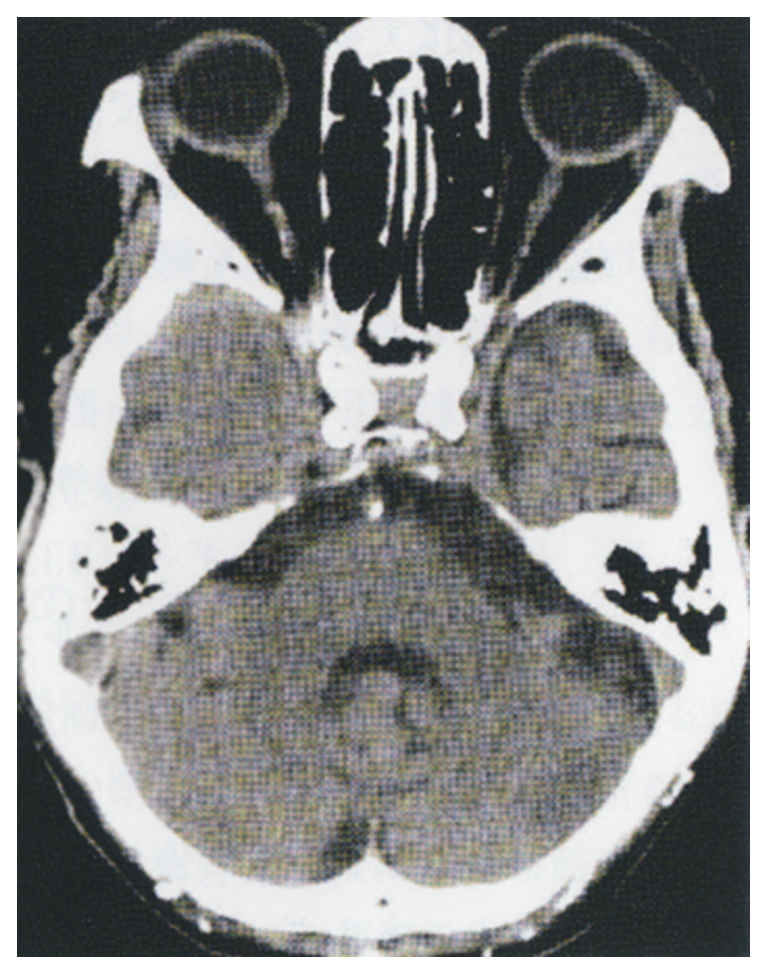
\includegraphics[width=5cm]{image/other/artifact_1_after.eps}
  \end{center}
  \vspace{-0.5cm}\hspace{2cm}
   (b)スペクトラルCT(70keV)
 \end{minipage}
 \begin{center}
  \vspace{-1zh}
  \caption{後頭蓋窩アーチファクトの低減\cite{spectralCT}:(a)には赤丸部に橋を横切るような線状の低吸収域が見られる。これにより脳幹や小脳などの描画不明瞭にとなりやすく,同部の出血や梗塞などの診断には限界がある。(b)ではこのアーチファクトが低減され,脳実質の観察が容易になる。}
  \label{fig:artifact_1}
  \end{center}
\end{figure}


\begin{figure}[H]
 \begin{minipage}{0.52\hsize}
  \begin{center}
   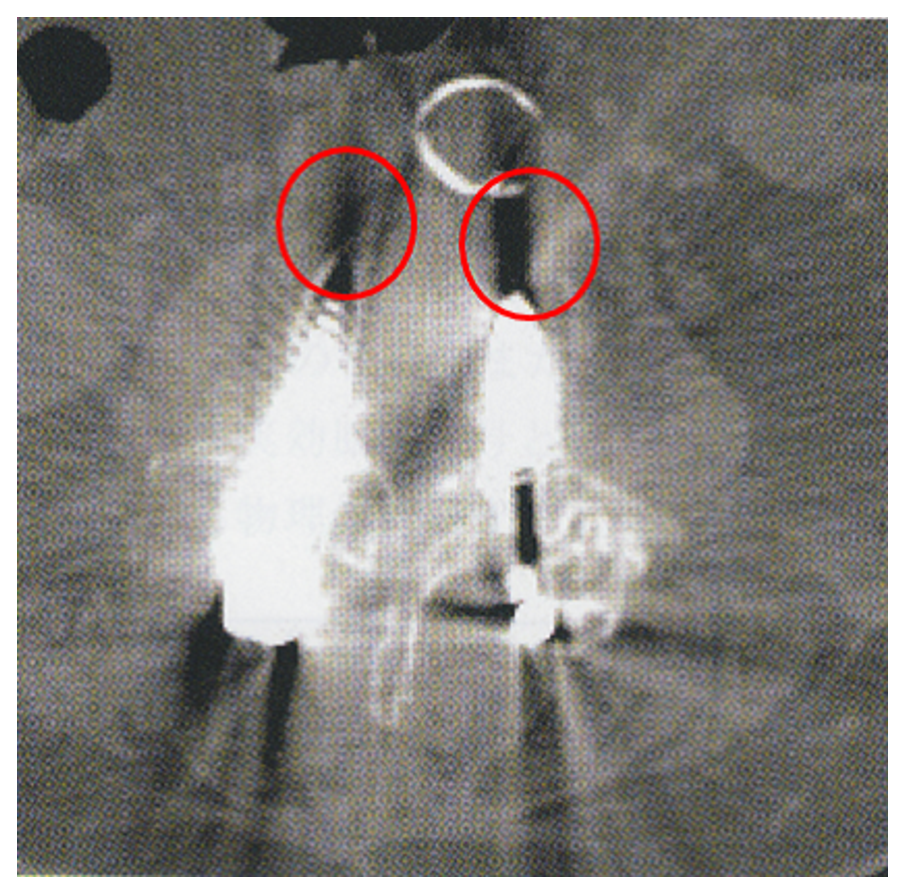
\includegraphics[width=5cm]{image/other/artifact_2.eps}
  \end{center}
  \vspace{-0.5cm}\hspace{1cm}
   (a)エネルギー積分型CT画像(140kVp)
 \end{minipage}
   \begin{minipage}{0.5\hsize}
  \begin{center}
   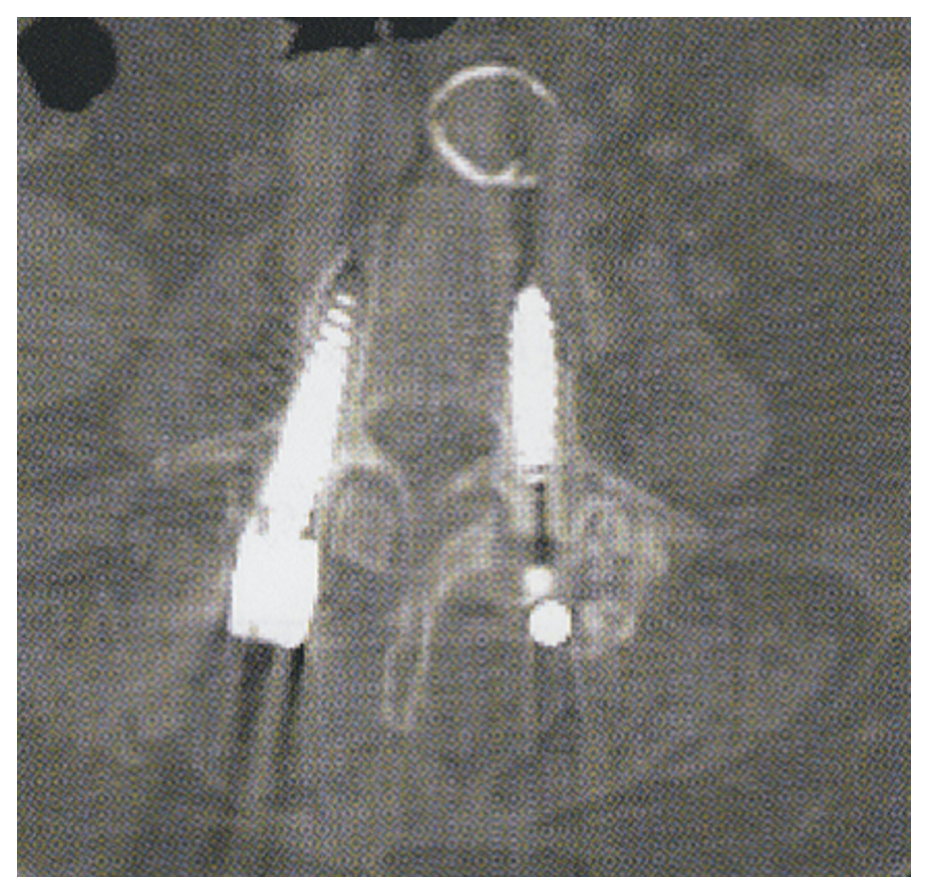
\includegraphics[width=5cm]{image/other/artifact_2_after.eps}
  \end{center}
  \vspace{-0.5cm}\hspace{2cm}
   (b)スペクトラルCT(70keV)
 \end{minipage}
 \begin{center}
  \vspace{-1zh}
  \caption{金属アーチファクトの低減\cite{spectralCT}:金属スクリューを用いた腰椎後方固定術後症例で(a)では金属アーチファクトのためスクリュー自体およびその周辺組織の評価が困難となっているが,(b)では金蔵アーチファクトが著明に低原子,周辺組織の評価が容易になる。}
  \label{fig:artifact_2}
  \end{center}
\end{figure}
\subsubsection{媒質の同定}
先述のように従来のエネルギー積分型のCTでは,線源弱係数は物質が異なっても密度によっては同一になる場合があり,パラメータは一つのCT値のみであったため正確な物質の弁別をすることができなかった。しかし,スペクトラルCTではいくつかのエネルギー帯においてCT値を取得することができるため,パラメータが複数になることで正確な材質の弁別が可能となる。例えば,ある領域に対して低エネルギーと高エネルギーによる線源弱係数を求めたとする。その比($\mu(E_{\rm Low})/\mu(E_{\rm High})$)の原子番号依存性は既知であり,対象組織の密度,厚さに依存せず原子番号のみに依存する。(\Fref{fig:rate}参照)。すなわち,低エネルギー領域と高エネルギー領域の線源弱係数の比を求めることによって,検査対象の組織の原子番号を求めることができる\cite{material_id}。\\
\ \ また,各エネルギー帯ごとに線源弱係数を求めた後,そのエネルギー依存性を既知の候補物質の線源弱係数のエネルギー依存曲線と比較することにより媒質を同定する手法もある\cite{ogawa_id}。



\subsubsection{軟部組織のコントラスト強調}
エネルギーごとに投影データを得て,これに対して重み付けを行うことによって,特定の媒質のコントラスト自由に変えることができる。\Fref{fig:material_atten}に示すようにX線光子のエネルギーが低いほど光電吸収が支配的になるので線源弱係数の物質間での差が高エネルギーより大きくなるので,低エネルギー画像に多く重みを付けることによりコントラストを強調することができる。特にこれは軟部組織のイメージングのように線源弱係数が低エネルギーのみでしか変化しないような場合に有効である\cite{kowase}\cite{ogawa_kaisetu}。

\begin{figure}[H]
 \begin{center}
 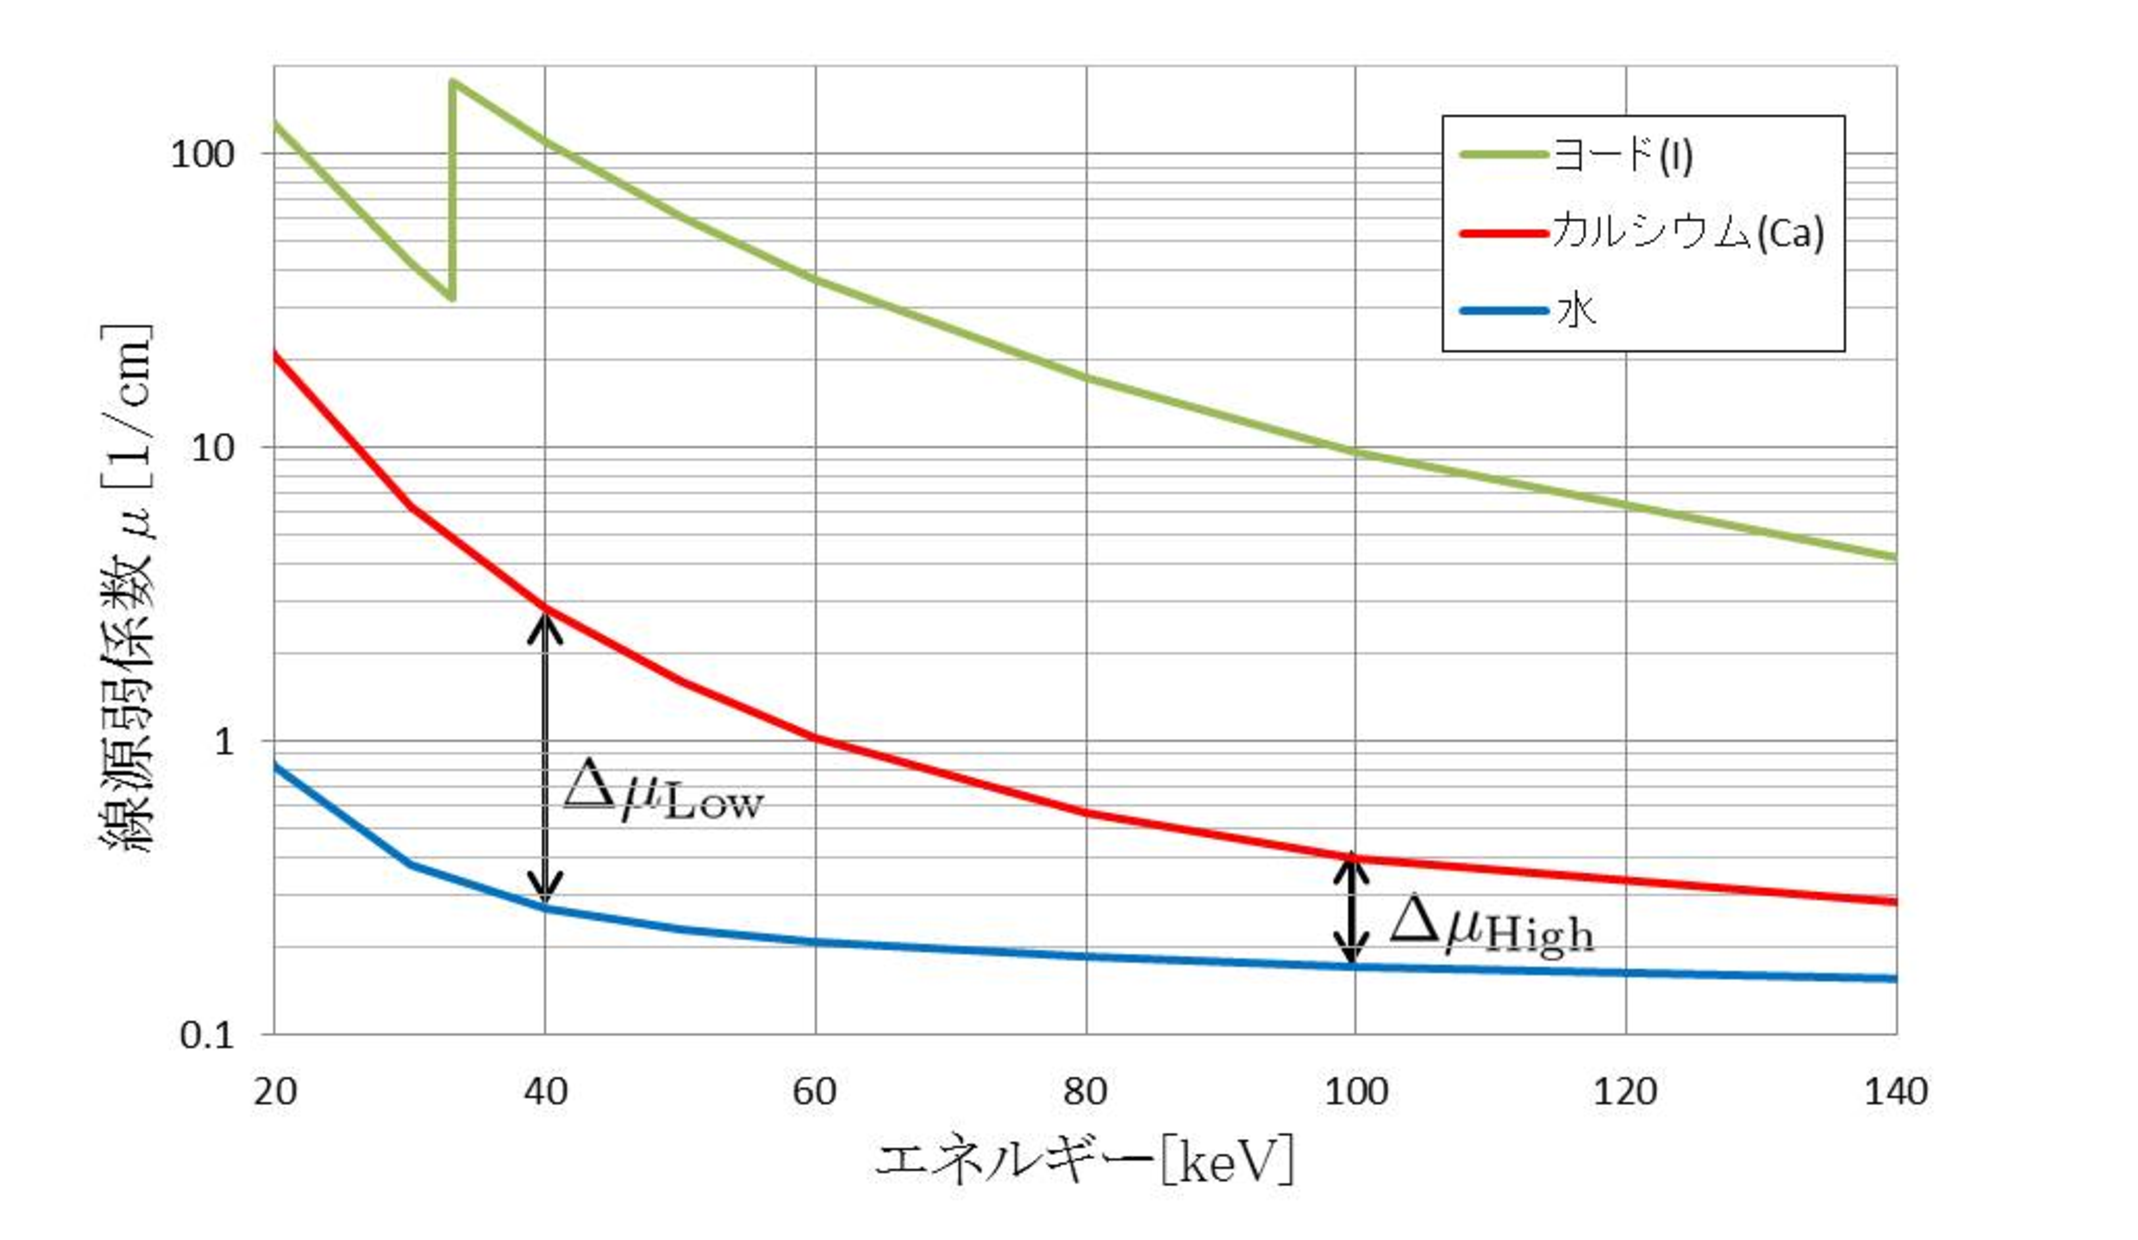
\includegraphics[width=10cm]{image/other/material_atten.eps}
 \end{center}
  \vspace{-0.7cm}
 \caption{ヨード,カルシウム,水の線源弱係数(NISTより作成)\newline $\Delta\mu_{\rm Low}$が$\Delta\mu_{\rm High}$より大きいため低エネルギーにおける画像の方がコントラストが強調される}
 \label{fig:material_atten}
\end{figure}


\subsubsection{ノイズの低減(SN比の向上)}
フォトンカウンティング方式にすることによって電子的なノイズを低減することができる。データの計測時には,アナログ系の電子的ノイズが混入し,その計測値に誤りを発生させるこになる。\Fref{fig:noise_affect}(a)は70kVのX線管から発生したX線の理想的なエネルギースペクトルと,ある量の水を透過した後のエネルギースペクトルを模式的に示したものである。実際の計測においては計測対象の透過X線は,X線発生時における統計的な変動,高圧や管電流の揺らぎの影響を受け,さらに計測時に混入する電子的ノイズによって\Fref{fig:noise_affect}(b)のようなスペクトルおを計測することになる。この時,従来のエネルギー積分型の計測を行うとそのノイズ成分は加算され影響を与えることになるが,フォトンカウンティング型ではエネルギー帯域ごとX線光子が個数としてカウントされるので,ノイズの影響は受けにくくなる。このような電子的ノイズが大きく影響を与えるのは,計数時のX線の強度が非常に小さくなる場合である。

\begin{figure}[H]
 \begin{center}
 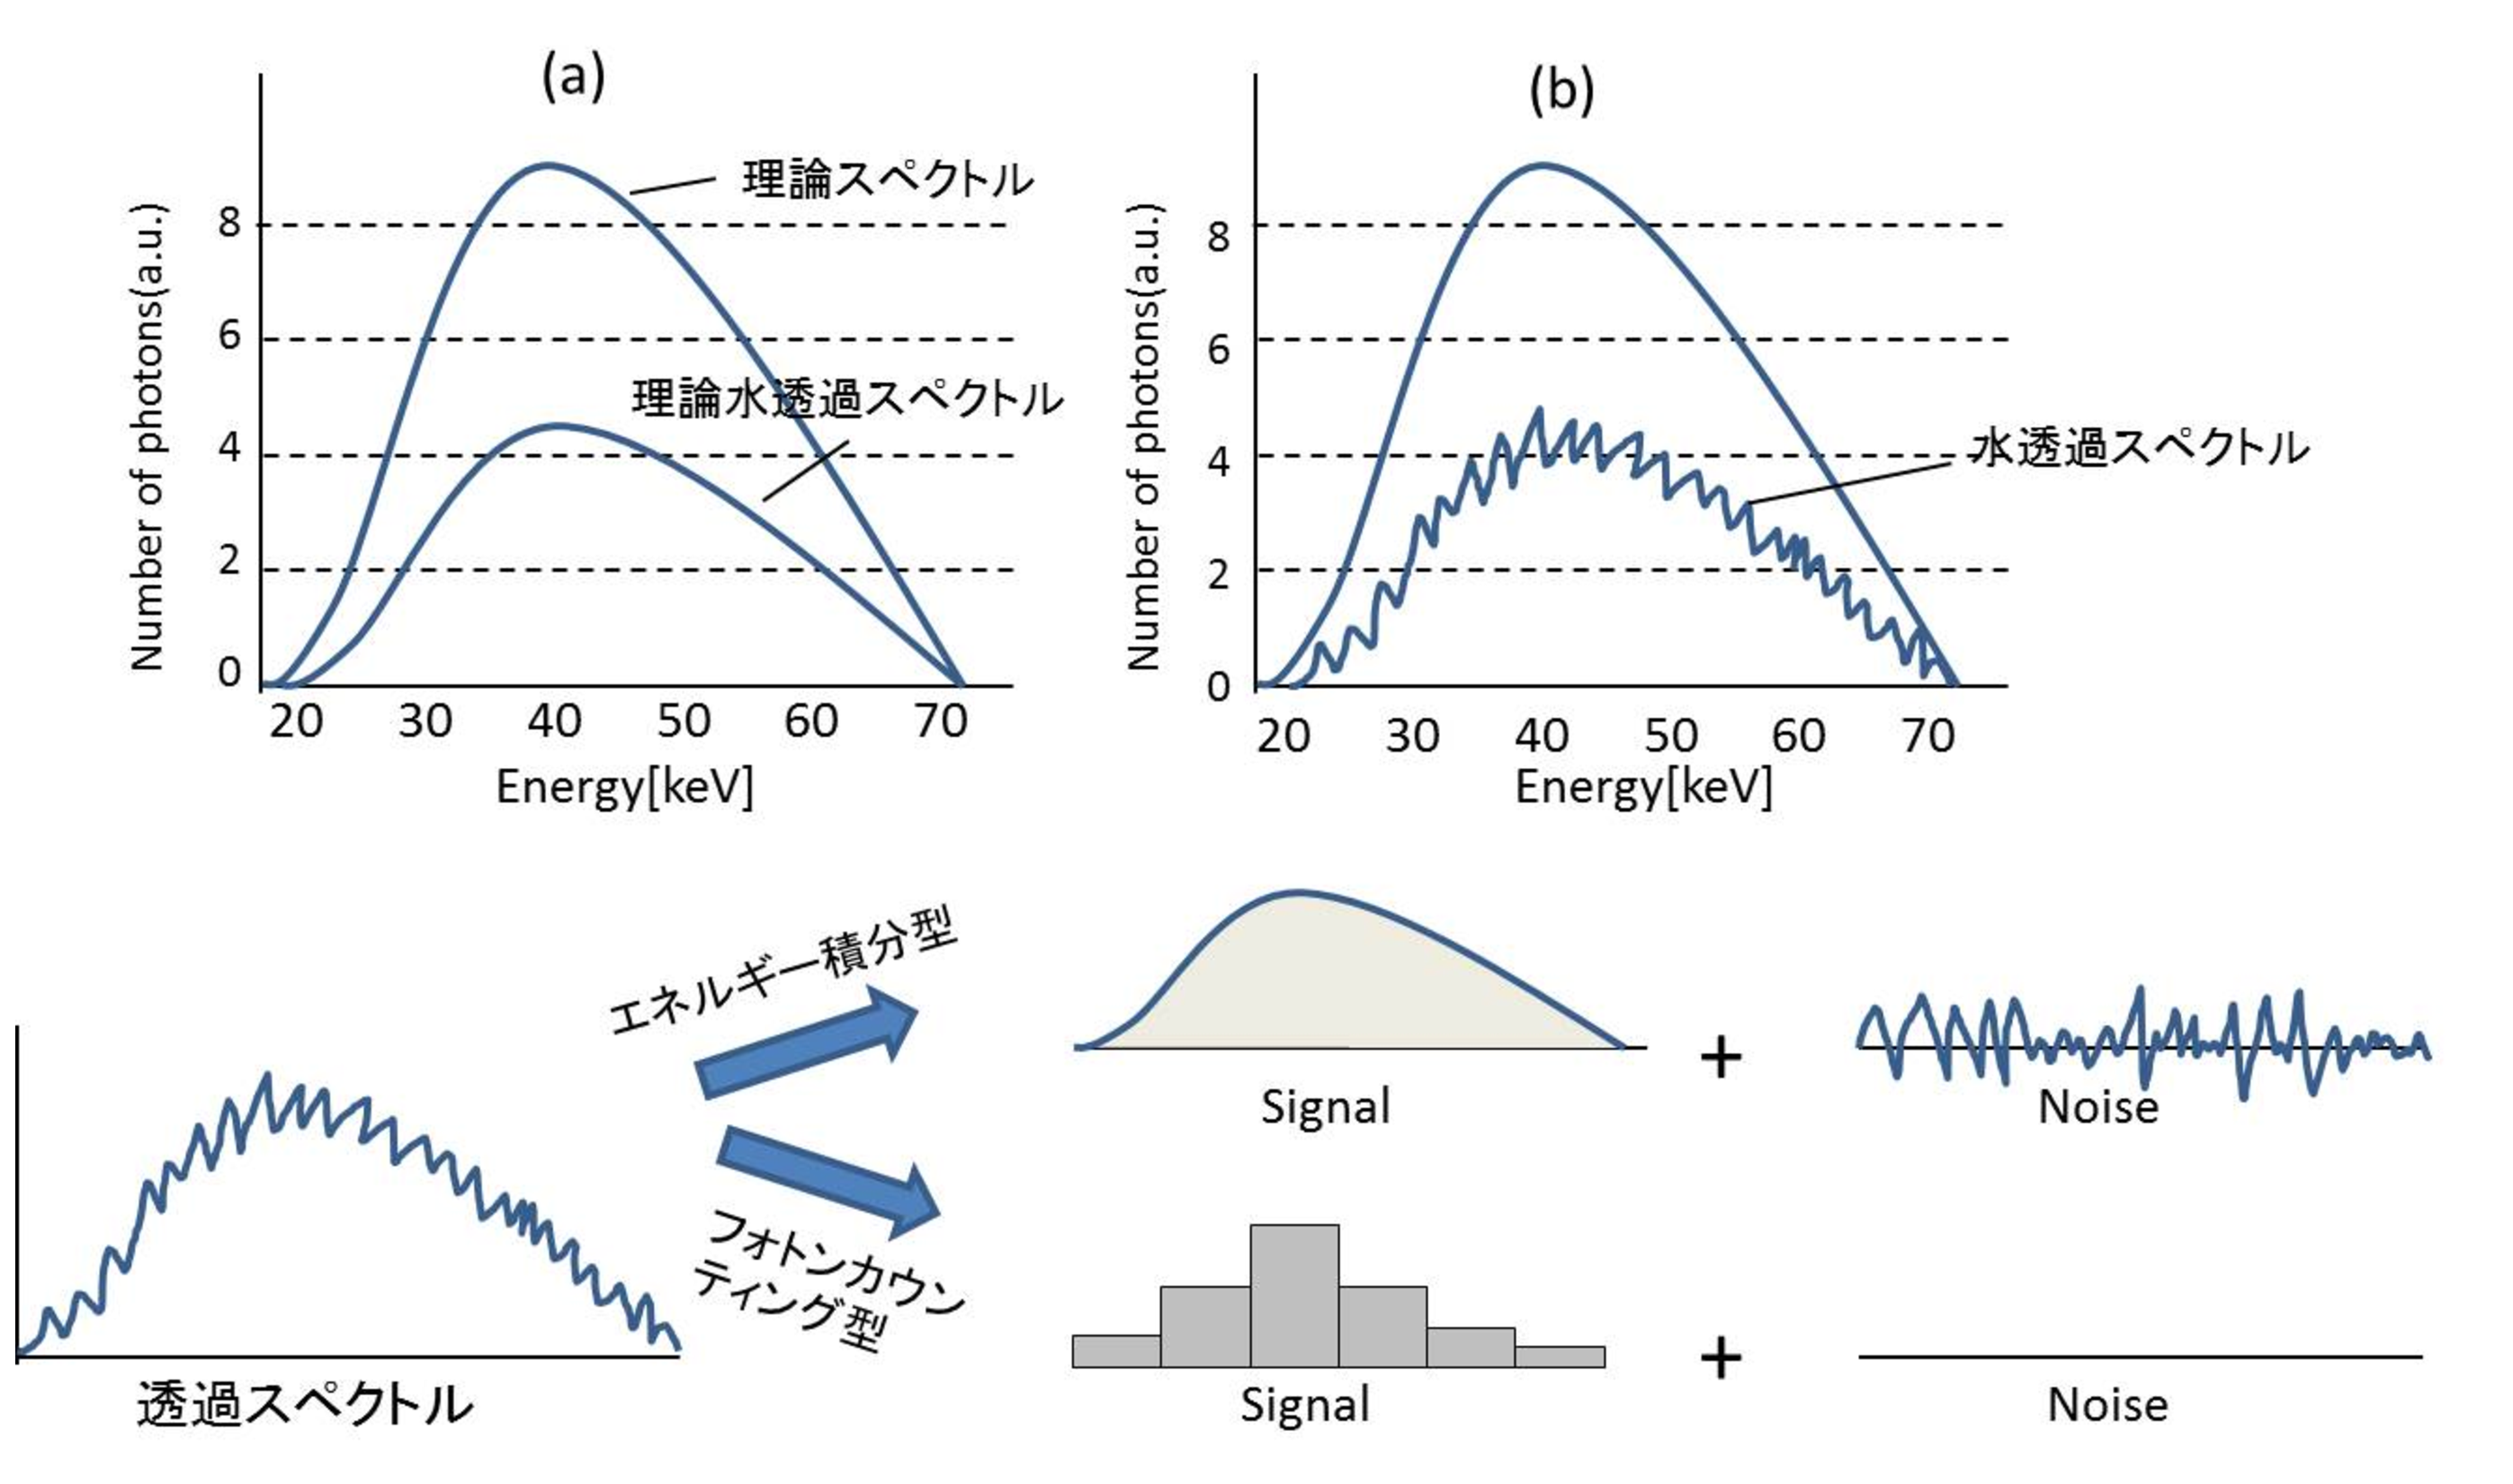
\includegraphics[width=12cm]{image/other/noise_affect.eps}
 \end{center}
 \caption{エネルギー積分型CTとスペクトラルCTにおけるノイズの影響の比較\cite{ogawa_kaisetu}}
 \label{fig:noise_affect}
\end{figure}

\subsubsection{k吸収端イメージング}
従来のエネルギー積分型の方式では実現できないイメージングがk吸収端イメージングである。人体を構成する元素の大部分は原子番号が非常に小さいため,k吸収端は低エネルギーレベルに存在するため,そのk吸収端を捉えることは不可能であるが,造影剤として用いるガドリニウム(Gd)やヨード(I)のk吸収端はそれぞれ50.2keV,33.2keVであり,k吸収端の前後でデータの計測を行うことで造影剤の分布を特異的に示すことができる。例えばGdの場合bin0:40-49keV,bin1:50-59keVとしそれぞれのbinでCT画像を再構成した後,bin1のCT画像からbin0のCT画像を引き算することにより,造影剤を含んだ血管や組織などの明瞭な画像下が可能となる。

\begin{figure}[H]
 \begin{center}
 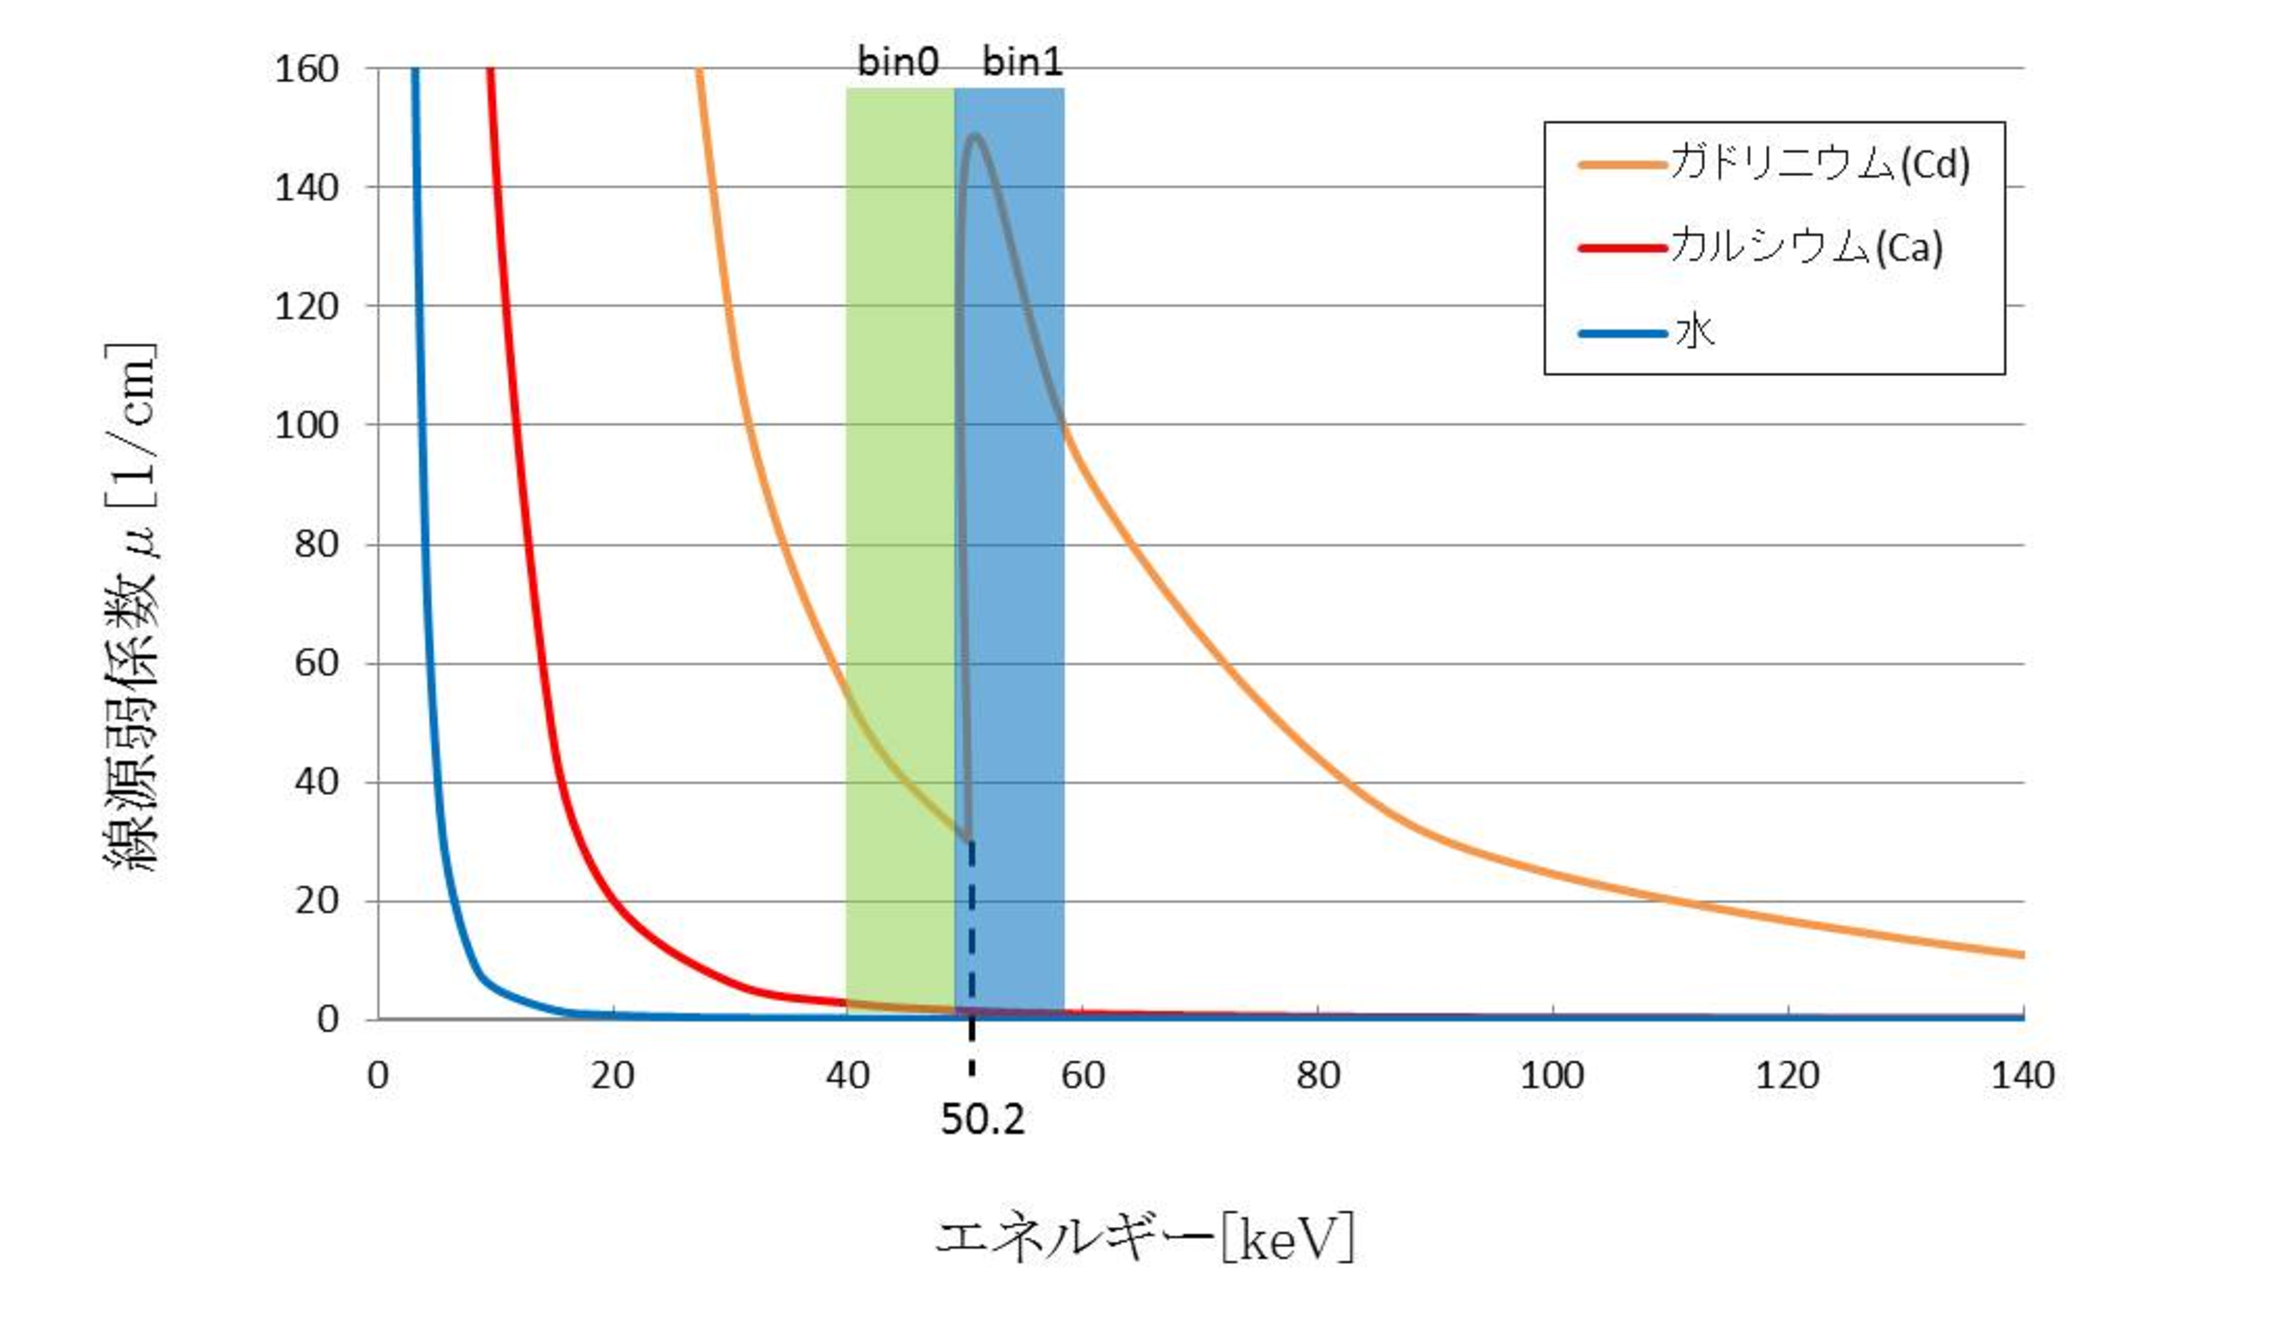
\includegraphics[width=12cm]{image/other/k-edge.eps}
 \end{center}
 \vspace{-0.7cm}
 \caption{k吸収端イメージングの原理(減弱曲線はNISTより作成)}
 \label{fig:k-edge}
\end{figure}









